
%% using aastex version 6
\documentclass[twocolumn]{aastex6}

% These are the available options:
%   manuscript	: onecolumn, doublespace, 12pt fonts
%   preprint	: onecolumn, single space, 10pt fonts
%   preprint2	: twocolumn, single space, 10pt fonts
%   twocolumn	: a two column article. Probably not needed, but here just in case.
%   onecolumn	: a one column article; default option.
%   twocolappendix: make 2 column appendix
%   onecolappendix: make 1 column appendix is the default. 
%   astrosymb	: Loads Astrosymb font and define \astrocommands. 
%   tighten	: Makes baselineskip slightly smaller
%   times	: uses times font instead of the default
%   linenumbers	: turn on lineno package.
%   trackchanges : required to see the revision mark up and print output
%   numberedappendix: Labels appendix sections A, B, ... This is the default.
%   appendixfloats: Needed. Resets figure and table counters to zero

\usepackage{verbatim}
\usepackage{amsmath}
\usepackage{graphicx}
\usepackage{cleveref}
\usepackage{hyperref}
\usepackage[normalem]{ulem}

\usepackage{xcolor}

\newcommand{\vdag}{(v)^\dagger}
\newcommand\aastex{AAS\TeX}
\newcommand\latex{La\TeX}
\newcommand{\rr}[1]{$r_{#1}$}
\newcommand{\M}[1]{$M_{#1}$}
\newcommand{\A}{\textit{A}}
\newcommand{\N}{\textit{N}}
\newcommand{\Pf}{$P_{F,0}$}
\newcommand{\Pn}{$P_{N,0}$}
\newcommand{\p}{$p_0$}
\newcommand{\tf}{$t_F$}
\newcommand{\tn}{$t_N$}
\newcommand{\feat}{`Featured'}
\newcommand{\notfeat}{`Not'}


%%%%%%%%%%%%%%%%%%%%%%%%%%%%%%%%%%%%%%%%%%%%%%%%%%%%%%%%%%%%%%
%% The following commented section outlines numerous optional output that
%% can be displayed in the front matter or as running meta-data.
%%
%% You can insert a short comment on the title page using the command below.
%% \slugcomment{Not to appear in Nonlearned J., 45.}
%%
%% If you wish, you may supply running head information, although
%% this information may be modified by the editorial offices.
%%\shorttitle{\aastex sample article}
%%\shortauthors{Schwarz et al.}
%%
%% You can add a light gray and diagonal water-mark to the first page 
%% with this command:
%% \watermark{text}
%% where "text", e.g. DRAFT, is the text to appear.  If the text is 
%% long you can control the water-mark size with:
%% \setwatermarkfontsize{dimension}
%% where dimension is any recognized LaTeX dimension, e.g. pt, in, etc.
%%
%%%%%%%%%%%%%%%%%%%%%%%%%%%%%%%%%%%%%%%%%%%%%%%%%%%%%%%%%%%%%%%%%%%


\begin{document}


\title{Galaxy Zoo EXPRESS: Integrating human and machine intelligence in morphology classification tasks}

%% Use \author, \affil, plus the \and command to format author and affiliation 
%% information.  If done correctly the peer review system will be able to
%% automatically put the author and affiliation information from the manuscript
%% and save the corresponding author the trouble of entering it by hand.
%%
%% The \affil should be used to document primary affiliations and the
%% \altaffil should be used for secondary affiliations, titles, or email.

%% Authors with the same affiliation can be grouped in a single
%% \author and \affil call.
\author{Melanie Beck, Claudia Scarlata, Lucy Fortson}%\altaffilmark{1}
\author{Chris Lintott}
\author{Melanie Galloway, Kyle Willett}
\author{Brooke Simmons}
\author{Karen Masters}
\author{Phil Marshall}

\affil{Department of Physics, University of Oxford, Oxford OX1 3RH}
\affil{Minnesota Institute for Astrophysics, University of Minnesota, Minneapolis, MN 55454}
%\altaffiltext{1}{AAS Journals Data Scientist}

%% Mark off the abstract in the ``abstract'' environment. 
\begin{abstract}

We implemented one of the first human-machine combos by running a kick ass
simulation on previous citizen science data in conjunction with machine algorithms. 
And guess what? We can obtain at least an ORDER OF MAGNITUDE improvement in the 
efficiency of classification. So we got that going for us. Which is nice. 

\end{abstract}

%% Keywords should appear after the \end{abstract} command. 
%% See the online documentation for the full list of available subject
%% keywords and the rules for their use.
\keywords{editorials, notices --- 
miscellaneous --- catalogs --- surveys}


\section{Introduction} \label{sec:intro}
The age of Big Data is upon us. Has been upon us. The astrophysics comnunity is 
already shifting focus, preparing for the way in which our science will change and 
the way in which we perform our science will chagne. Look at the new CasJobs -- 
This is the type of shit we need: where analytical tools are integrated at the source
of the data repository. Downloading datasets is a thing of the past. you can't do 
Big Data science if you have to constantly move dem data around. 

Another area we need to get ready for is how we label all that shit in the sky. 
We absolutely love labelling things and it's damn necessary too! And the more sky
we see both in terms of area and depth is going to grow huge AF. We need to find 
efficient, clever ways of picking out transients, radio shits, gravitational lenses, 
galaxy morphology, .... make a really big list with things that are rare or common
or time-domain-y. LSST, Euclid, WFIRST are going to swamp us. 

In this paper we consider the particular problem of galaxy morphology. This 
challenge is actually several combined because it necessitates the need to 
identify the mundane from the unique or rare and, ideally, requires an incredible
amount of detail in order to withdraw useful science. Additionally, morphology is
a great place to start because we can already begin to plan for the future by 
considering the Data of Today. The imaging techniques of future surveys will 
change mostly in resolution and depth; things we can account for. 

Another great reason to use morphology as an example is that we can draw on 
vast, well-established citizen science projects which have contributed to several 
past publications and have lead to serenditious discovery on multiple occasions. 
There is no doubt that to spurn this resource would be a disservice to science!!!!

So then. Morphology it is. And don't think that morphology is just a waste of time
either. While there is certainly always room for improvement in our classification 
system including the fact that our categories were made up 100 years ago and only 
work for the local universe... putting galaxies into categories helps us learn 
about the way dem galaxies be living their lives. 

%%%-------------------------------------------------------
%%% FIGURE:     GZ EXPRESS Schematic
%%%-------------------------------------------------------
\begin{figure*}[ht!]
%\figurenum{1}
\plotone{figures/GZExpress_schematic_newlayout_v3.png}
\caption{Schematic of our hybrid system. Human classifiers are shown images of galaxies via the Galaxy Zoo web interface. These  classifications are recorded and processed according to section XXX. As a result of the processing, those subjects whose probabilties cross the classification thresholds are passed to the machine classifier as a training sample. The trained machine is then applied to the remaining subjects in the database (test sample). Those subjects which the machine classifies with high confidence are removed from the sample and considered fully classified. The rest remain in the database to be seen by human classifiers. \label{fig: schematic}}
\end{figure*}

The idea of combing human and machine classifications IS NOT NEW. That shit's
old AF and a big topic of study in computer science circles; circles we astronomers
have never been invited to but of which we should still be aware. \textbf{Citations
from Chris go here!} So this idea is not novel. What IS novel is one of the first practical
applications and the ability to explore the repercussions of such a system by 
simulating various outcomes on previously collected data. 


In this paper we consider visual classifications from both citizen scientists through
the use of Galaxy Zoo data as well as expert visual classifications from various 
published catalogs as well as visual classifications from within our own team. We 
will combine these with various parameters which originally sought to automatically
classifiy galaxy morphology. parameters like the Gini coefficient, M20, CAS, etc. 
We'll wrap this all up in a neat little package by throwing it all in the 
supervised machine learning algorithm black box which I'll actually explain.
And out will pop some sweet classifications! 

With all that said, start the paper! Section blah will be the components of the method. Section blah will be detail about post-processing visual classifications. Section blah will be about the machine algorithm. Section blah will be testing the method in various circumstances. Section blah will be results. Section blah will be Discussion/Conclusions. 





\section{Galaxy Zoo Express Overview}
In Galaxy Zoo Express (GZX) we combine humans and machines with the goal of 
increasing galaxy morphology classification efficiency, both in terms of the rate 
of classification over time and in the amount of human effort required. 
Figure~\ref{fig: schematic} presents a schematic of GZX which includes section 
numbers as a shortcut for the savvy reader. We note that transparent portions
 of the schematic represent areas of future work which we explore in section~\ref{sec: visions}. 

Any system combining human and machine classifications will have a set of generic 
features: a group of human classifiers, at least one machine classifier, and a 
decision engine which determines how these classifications should be combined.


We draw from the Galaxy Zoo 2 (GZ2) classification database which allows us to 
 create simulations of human classifiers (described in section~\ref{sec: data}).
These classifications are used most effectively when processed with SWAP, 
a Bayesian code described in  section~\ref{sec: SWAP}, first developed for the 
Space Warps gravitational lens discovery project. 
These subjects become the basis for the machine's training sample. 

In section~\ref{sec: machine} we incorporate a machine classifier; where, for this
project, we have developed a random forest classifier which trains on easily measured 
physical parameters such as Concentration, Asymmetry, Gini coefficient and M$_{20}$ as input. 
After a batch of (human) classifications is processed,  the machine is trained and 
its performance assessed against a validation sample. This procedure is repeated and 
the machine grows in accuracy as the size of the training sample increases (to a point). 
Once the machine reaches an acceptable level of performance it is run against the 
remaining galaxy sample. Images reliably classified by machine are not further classified by humans.

Even with this simple description, one can see that the classification process 
will progress in three phases. At first, the machine will not yet have reached the 
acceptable level of performance and the only subjects classified
 are those for which human classifiers have reached consensus. 
Secondly, the machine will rapidly improve and both humans and machine will be 
responsible for classification. Finally, improvement in the machine performance 
will slow and the remaining images will likely need to be classified by humans (if they can be 
classified at all). These results are explored in section~\ref{sec: results}. 
This blueprint allows even moderately successful machine learning 
routines to make significant contributions alongside human classifiers and 
removes the need for ever-increasing performance in machine classification.



%%----------------------------------------------------------------------------------------------------------------------------------------------------
%%   Galaxy Zoo 2 Data Description
%%----------------------------------------------------------------------------------------------------------------------------------------------------
\section{Galaxy Zoo 2 Classification Data} \label{sec: data}

Our simulations utilize original classifications made by volunteers during the GZ2 project. 
These data are described in detail in~\cite{Willett2013} though we provide a brief overview here.  
The GZ2 subject sample was designed to consist of the brightest 25\% ($r$ band magnitude $< 17$) 
of galaxies residing in the SDSS North Galactic Cap region from Data Release 7 
and included both subjects with spectroscopic and photometric redshifts out to $z < 0.25$.
In total, 285,962 subjects were classified in the GZ2 Main Sample 
catalogs\footnote{data.galaxyzoo.org} . 
Of these, 243,500 have spectroscopic redshifts while 42,462 have only photometric redshifts.  

Subjects were shown as color composite images via a web-based interface wherein 
volunteers answered a series of questions pertaining to the morphology of the subject.
With the exception of the first question, subsequent queries were 
dependent on volunteer responses from the previous task creating a complex decision tree. 
Using GZ2 nomenclature,  a \textit{classification} is defined as the total amount of
information about a subject obtained by completing all tasks in the decision tree. 
A \textit{task} represents a segment of the
tree consisting of a \textit{question} and possible \textit{responses}. 
A subject is \textit{retired} after it has achieved a sufficient amount of classification.


For the analysis in this paper we utilize the first task in the tree, 
`Is the galaxy simply smooth and rounded, with no sign of a disk?' to which possible 
responses include `smooth', `features or disk', or `star or artifact'. This choice
serves two purposes: 1) this question is one of only two questions in the GZ2
decision tree that is asked of every subject thus maximizing the amount of data
we can work with, and 2) our analysis will assume a 
binary task and this question is simple enough to mold into such a form. 

To force such a binary classification, we group `star or artifact' responses with `features or disk'. 
Additionally, we define a set of `true' labels for each GZ2 subject to which
we can compare labels assigned by Galaxy Zoo Express (GZX).  
The GZ2 catalog assigns every subject three types of volunteer vote fractions: 
raw, weighted, and debiased. 
Debiased vote fractions are calculated to correct morphological classifications
for redshift bias, a task that GZX is not yet built to handle. 
The weighted vote fractions serve to downgrade malicious volunteers and bots, 
a task we perform as well. However, because the mechanism for
determining malicious volunteers is entirely different between GZ2 and GZX, 
we use GZ2 raw vote fractions as the closest comparison. 
Specifically, we take the majority raw vote fraction as the label for that subject. If the 
majority resided under `star or artifact' or `feature or disk', it was labeled as \feat; 
otherwise it was labeled~\notfeat. We note that only 512 subjects in the GZ2 
catalog have a majority `star or artifact' vote 
fraction, contributing less than half a percent contamination. 

In total, the data consist of over 16 million classifications from 83,943 individual volunteers. 
As we discuss in Section~\ref{sec: SWAP}, the software we use requires that every 
volunteer see a subset of subjects that are expertly identified by a member of the GZ team. 
We thus utilize only those classifications made by one of the 30,894 volunteers that 
identified one or more of our gold standard sample (see Section~\ref{sec: training sample}). 
We note that these volunteers represent 36\% of all users 
yet provide nearly 90\% of the total Galaxy Zoo classification data, 
reducing the total number of classifications to approximately 14 million.





%%----------------------------------------------------------------------------------------------------------------------------------------------------
%%   Talk About SWAP 
%%----------------------------------------------------------------------------------------------------------------------------------------------------
\section{Efficiency through clever human-vote processing}\label{sec: SWAP}

Galaxy Zoo requires a large number of independent classifications for each subject and
 this value is typically set at forty individual volunteer classifications. 
Once a project reaches completion,~\cite{Willett2013} down-weight inconsistent 
and unreliable volunteers.  
While this process reduces input from malicious users and `bots', 
it doesn't reward consistent volunteers. Furthermore, waiting until project completion 
doesn't allow for efficient utilization of super-users, those volunteers who are 
exceptional at classification tasks.

As a first step towards increasing classification efficiency, we instead employ 
software adapted from the Space Warps Zooniverse project~\citep{Marshall2016} 
which searched for and discovered several gravitational lens 
candidates in the CFHT Lensing Survey (cite XXX).  Dubbed SWAP (Space Warps Analysis Pipeline),  
the software predicted the probability that an image contained a gravitational lens given 
volunteers' classifications as well as their past experience. We provide a brief overview here.  

The software assigns each volunteer an \textit{agent} which interprets that volunteer's 
classifications. Each agent assigns a 2 by 2 confusion matrix to their volunteer which encodes
that volunteer's probability of correctly identifying feature `\A'  given that the subject 
actually exhibits feature \A, and the probability of correctly identifying
the absence of feature \A~(denoted as \N) given that the subject does not exhibit 
that feature. The agent updates these probabilities by estimating them as 

\begin{equation}
P(``X" | X, d) \approx \frac{N_{``X"}}{N_{X}}
\end{equation}
where $N_{``X"}$ is the number of classifications the volunteer labeled as type $X$, 
$N_X$ is the number of subjects the volunteer has see that were actually of type $X$,
and $d$ represents the history of the volunteer (all subjects they have seen). 
The software employs two prescriptions for when the 
agent updates the volunteer's confusion matrix. In \textit{Supervised} mode the 
probabilities are only updated after the volunteer identifies a training subject.
In \textit{Supervised and Unsupervised} mode, the agent
updates the probabilities after every subject the volunteer identifies.  

In addition to agent probabilities, each subject begins with a prior probability 
that it exhibits feature \A: $P(A) = p_0$. 
When a volunteer makes a classification $C$, Bayes' Theorem is used to derive how 
the agent should update the subject's prior probability into a posterior: 

\begin{equation}
P(A|C) = \frac{ P(C|A) P(A) }{P(C|A) P(A) + P(C|N) P(N)}
\end{equation}
where this value can then be calculated using the elements of the agent's 
confusion matrix. \cite{Marshall2016} show that perfect volunteers (i.e., those 
with $P(``A"| A) = 1.0$ and $P(``N" | N) = 1.0$ would calculate the posterior
probability of the subject to be $1.0$ which is not surprising (perfect classifiers 
are perfect!). However, they also show that \textit{obtuse} classifiers (those with 
$P(``A" | A) = 0.0$ and $P(``N" | N) = 0.0$ also produce a posterior probability 
of $1.0$; demonstrating that obtuse volunteers are just as helpful as perfect volunteers.

As the project progresses, each subject's prior probability is continually updated 
and is nudged to higher or lower probability depending on volunteer classifications.
Probability thresholds can then be set such that subjects crossing these thresholds 
are highly likely to exhibit the feature of interest (or highly unlikely!). While most subjects
will cross a classification threshold, not all do. In particular, subjects for 
which volunteers are unsure will simply bounce back and forth in probability space indefinitely. 
Those that do cross a threshold are considered \textit{retired}. The software no
longer records volunteer information on these subjects. 



\subsection{Volunteer Training Sample}\label{sec: training sample}

A key feature of the original Space Warps project was the training of 
individual volunteers through the use of simulated lensed galaxies. Volunteers were 
shown these simulated images interspersed with actual data with the simulated data shown
predominately at the beginning of the project. After a volunteer submitted their 
classification, the system provided feedback in the form of a pop-up comment. 
In this section we describe how we engineer the GZ2 data to mimic the Space 
Warps setup as closely as possible, though we note that retroactively training 
volunteers in real time is obviously not possible. 

We found that the SWAP software does not perform well without the use of designated 
training images. Furthermore, the software requires that these training images
be introduced at the beginning of the project to allow volunteer confusion matrices
to update sufficiently before intense classification of test images commences. 
To mimic this behavior we select a sample of $\sim$3500 SDSS galaxies which 
overlaps the \cite{NairAbraham2010} catalog. This catalog contains $\sim$14K 
galaxies expertly classified into various TTypes. Though helpful, this particular
classification isn't directly comparable to GZ2.   Instead, we reclassified the subsample 
amongst the Galaxy Zoo science team by building a small project on the Zooniverse
platform. The question posed to our science team was identical to the original 
question posed to the volunteers. Approximately 15 members of the GZ science team
contributed to these classifications and at least five experts saw each galaxy. Experts 
this case range from advanced graduate students, post docs, and several 
seasoned faculty members. Once
classification was complete, the votes were aggregated and a simple majority was 
used to provide expert label  to the 3500 subjects. 

While 3500 subjects is a sizable sample, not  every volunteer saw at least 
one of these ad-hoc training images. Because we wish to recreate the conditions 
of the Space Warps project, we remove from our data all volunteers who never 
classify at least one of these 3500 subjects. This reduces our raw data set from
16 million clicks to 14 million; from 90K unique volunteers to 30K. 

Finally, the classifications for these particular subjects could 
have timestamps anywhere within the 14-month time span during which the original project ran.
We therefore adjust the order of the classification timestamps such that 
annotations of training sample subjects
have timestamps well before all other GZ2 subjects. Since it is implicitly assumed
that a subject's classifications are independent and random, the order of the 
classifications should have a small effect, if any, on the results.  
When running a simulation, which pulls from the database according to timestamps,
the training image classifications are the first to be processed with SWAP.  


%% -------------------------------------------------------------------------------
%%   FIGURE:  VOLUNTEER PROBABILITIES
%% -------------------------------------------------------------------------------
\begin{figure}[t!]
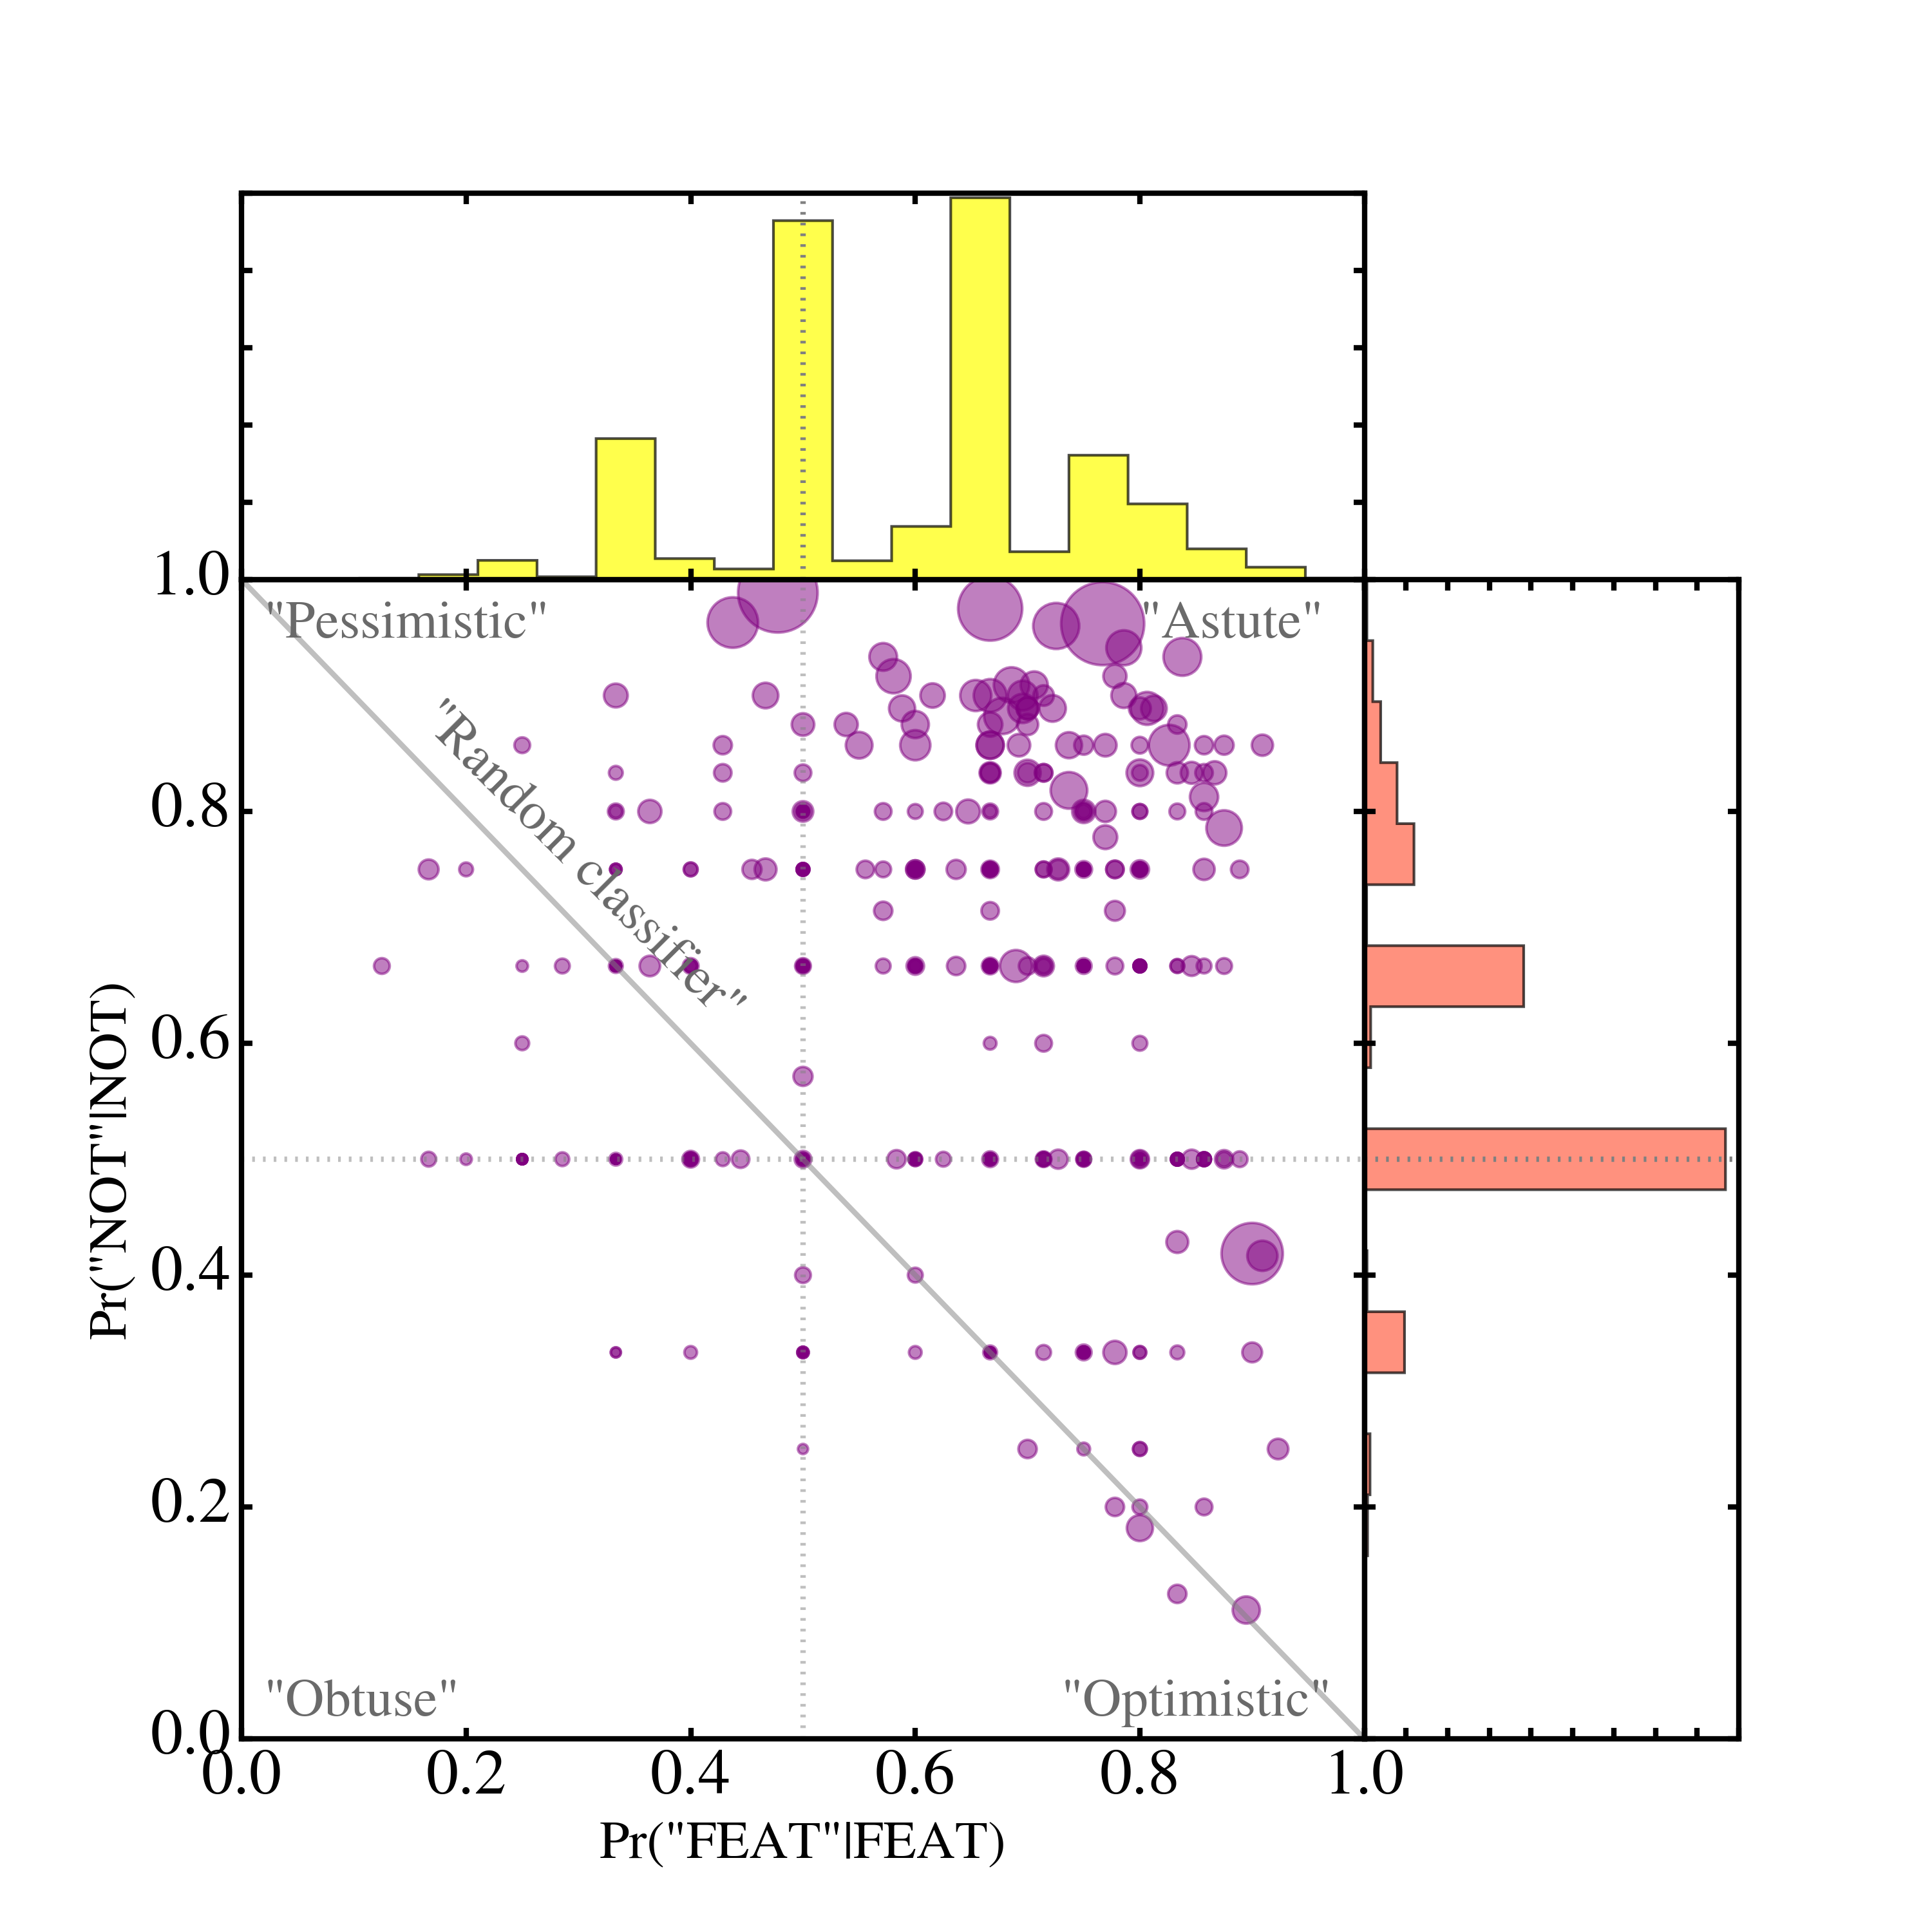
\includegraphics[width=3.7in]{figures/test_user_probs.png}
\caption{Volunteer probabilities for our fiducial SWAP run.  \label{fig: volunteer training}}
\end{figure}

%%%-------------------------------------------------------
%%%  FIGURE:    SWAP FIDUCIAL RUN
%%%-------------------------------------------------------
\begin{figure*}[ht!]
\plotone{figures/GZX_eval_and_retirement_baseline_4paper.png}
\caption{Fiducial SWAP simulation demonstrating the dramatic increase in the subject retirement rate as a function of GZ2 project time (in light blue) compared with the original GZ2 project (dark blue) corresponding to the left hand axis. Not only is efficiency increased by nearly an order of magnitude, we maintain high quality classifications as shown by high marks in accuracy, completeness and purity which correspond to the right hand axis.  Specifically, these metrics are computed on the sample obtained \textit{by that day in GZ2 project time}, e.g. on day 20, these metrics are computed on the 120K subjects which SWAP has classified by that time; their SWAP labels being compared to `true' labels derived from published GZ2 data. \label{fig: fiducial run}}
\end{figure*}

Figure~\ref{fig: volunteer training} demonstrates the volunteer training we achieve
with this scheme (figure adapted from~\cite{Marshall2016}). 
This figures shows the achieved confusion matrices for 1000 volunteers
where the size of the circle is proportional to the number of training images each
volunteer saw. Most of our volunteers fall into the `Astute' category indicating
they are exceptional at correctly identifying both `Featured' and `Not' (smooth) subjects. 
The full distribution of each probability for all volunteers can be seen in the 
histograms. The spikes at $p=0.5$ for each distribution indicate that of those
volunteers who saw only one subject (say,~\feat), their probability in the 
other (\notfeat) remains unchanged.


%%----------------------------------------------------------------------------------------------------------------------------------------------------
%%   Subsection: specifics of SWAP in context of simulations (sans Machine)
%%----------------------------------------------------------------------------------------------------------------------------------------------------
\subsection{Fiducial SWAP simulation}\label{sec: fiducial}

To simulate a live project we run SWAP on a regular timestep which we set as $\Delta t = 1$ day. 
At each timestep, the software pulls from the database all volunteer classifications which
have timestamps within that range. We cycle through three months of GZ2 classification data 
for each simulation we discuss below. However, before a simulation can be run, a number 
of parameters which control the behavior of SWAP must first be chosen. These include
 the initial confusion matrix assigned to each volunteer, the retirement
thresholds, and the prior probability of the subject. Specifically, we must choose 
\begin{itemize}
\item \Pf, the initial probability that a volunteer identifies a subject as being~\feat, $P_0(``F"|F)$
\item \Pn, the initial probability that a volunteer identifies a subject as being~\notfeat, $P_0(``N"|N)$
\item \p, the prior probability of a subject to be~\feat.
\item \tf, the threshold defining the minimum probability for a subject to be retired as~\feat.
\item \tn, the threshold defining the maximum probability for a subject to be retired as~\notfeat.
\end{itemize}


We begin with a fiducial simulation in which we set~\Pf, \Pn, and~\p~equal to $0.5$.
We let $t_F = 0.99$ and $t_N = 0.004$. 

Because our ultimate goal is to increase the efficiency of galaxy classification,
we consider the cumulative number of retired subjects
as a function of the original GZ2 project time for both the original GZ2 project
and the SWAP output. 
GZ2 retirement was defined by the number of volunteer classifications, requiring
$\sim$40 individual volunteers to reach classification consensus for each subject. 
We use a more lenient definition and consider a subject GZ2-retired after it achieves 
just 30 volunteer votes. SWAP retirement is determined by a subject's posterior 
probability crossing either of the retirement thresholds defined above. 

On the other hand, we don't want to prioritize efficiency at the expense of quality. 
Towards this end, we also consider the quality metrics of accuracy, 
purity and sample completeness as a function of GZ2 project time.  These are 
defined in the standard way where accuracy is the number of correctly
identified subjects divided by the total number retired; completeness is the number of 
correctly identified~\feat~subjects divided by the number of actual~\feat~retired; 
and purity is the number of correctly identified~\feat~subjects divided by 
the number of subjects retired as~\feat. 

Using as truth the labels we defined in section~\ref{sec: data}, we compute
these metrics on the subject set retired \textit{by that day of the GZ2 project.} 
For example, as shown in Figure~\ref{fig: fiducial run}, 
on the 20th day of the GZ2 project, 
SWAP has retired 120K subjects. Comparing those SWAP labels to their GZ2 labels, 
we find that the sample is 96\% accurate, nearly 100\% complete (that is, of all
the subjects we retire up to that point, we successfully identify all that are~\feat),
and 92\% pure. 


Figure \ref{fig: fiducial run} shows the results of our fiducial SWAP simulation
compared to the original GZ2 project. The right hand  axis shows the cumulative
number of retired subjects as a function of GZ2 project time. After 90 days, GZ2 
retires ~50K subjects while SWAP retires more than 225K. In other words, we classify 80\% of
the entire GZ2 sample in three months. The original GZ2 project took approximately
a year to complete. We thus achieve nearly an order of magnitude increase in
classification time. One can also consider the amount of human effort necessary to 
perform these classification tasks. Our SWAP run required $2.3 \times 10^6$ volunteer
votes to retire these 225K subjects. GZ2 required nearly $10 \times 10^6$ for the 
exact same subject set. Again, this is nearly an order of magnitude reduction in 
the human effort required to classify this data set! This reduction in human effort 
can be seen directly in Figure~\ref{fig: swap vote distributions} which shows the volunteer 
vote distributions achieved through SWAP (light blue) compared to GZ2 (dark blue)
for the $\sim$225K retired subjects. GZ2, as expected, has a distribution that peaks 
around $\sim$45 unique volunteers classifying each subject with 99\% of subjects 
having at least 25 classifications~\citep{Willett2013}. 
SWAP, on the other hand, has a distribution which peaks around 10 classifications
before retirement indicating that most subjects don't need as much human effort
to reach a sufficient level of consensus. Some subjects are `easy' to classify and can be 
retired in as few as 3 classifications, while subjects with less consensus will 
take more classifications, each one kicking the subject back and forth in probability space
before it eventually crosses one of the retirement thresholds. 
This explains the tail towards higher classifications requirement.

%%%-------------------------------------------------------
%%%  FIGURE:   SWAP vote distributions
%%%-------------------------------------------------------
\begin{figure}[t!]
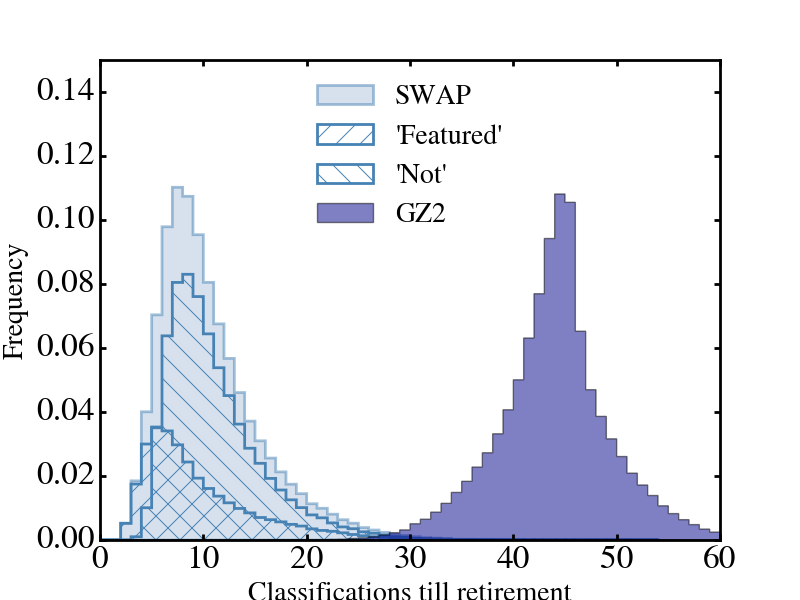
\includegraphics[width=3.65in]{figures/GZX_clicks_till_retired_baseline.png}
\caption{SWAP requires less human effort than GZ2 as evidenced by comparing the number of classifications until retirement for the $\sim$225K subjects retired by both SWAP and GZ2. GZ2 requires $\sim$45 classifications per subject before retirement. In contrast, most subjects only need approximately 10 classifications until retirement when processing volunteer votes with SWAP. Overall, SWAP can retire the same number of subjects but with an order of magnitude less human effort.  \label{fig: swap vote distributions}}
\end{figure}



 It is obvious that by clever and adaptive processing of volunteer classifications, 
efficiency of subject classification and retirement can be increased by an order of magnitude. 
However, the exact nature of subject retirement and associated quality metrics will
be, in part, a function of initial SWAP parameters. We now turn to a discussion of 
how classification and retirement change as a function of SWAP input parameters. 


%% ----------------------------------------------------------------------------------------------------------------------------------------------
%% DISCUSSION OF CHANGING SWAP PARAMETERS
%% ----------------------------------------------------------------------------------------------------------------------------------------------
\subsection{Exploring SWAP's Parameter Space}


%% -------------------------------------------------------------------------------
%%   FIGURE:  SWAP -- adjust CONFUSION MATRIX
%% -------------------------------------------------------------------------------
\begin{figure}[t!]
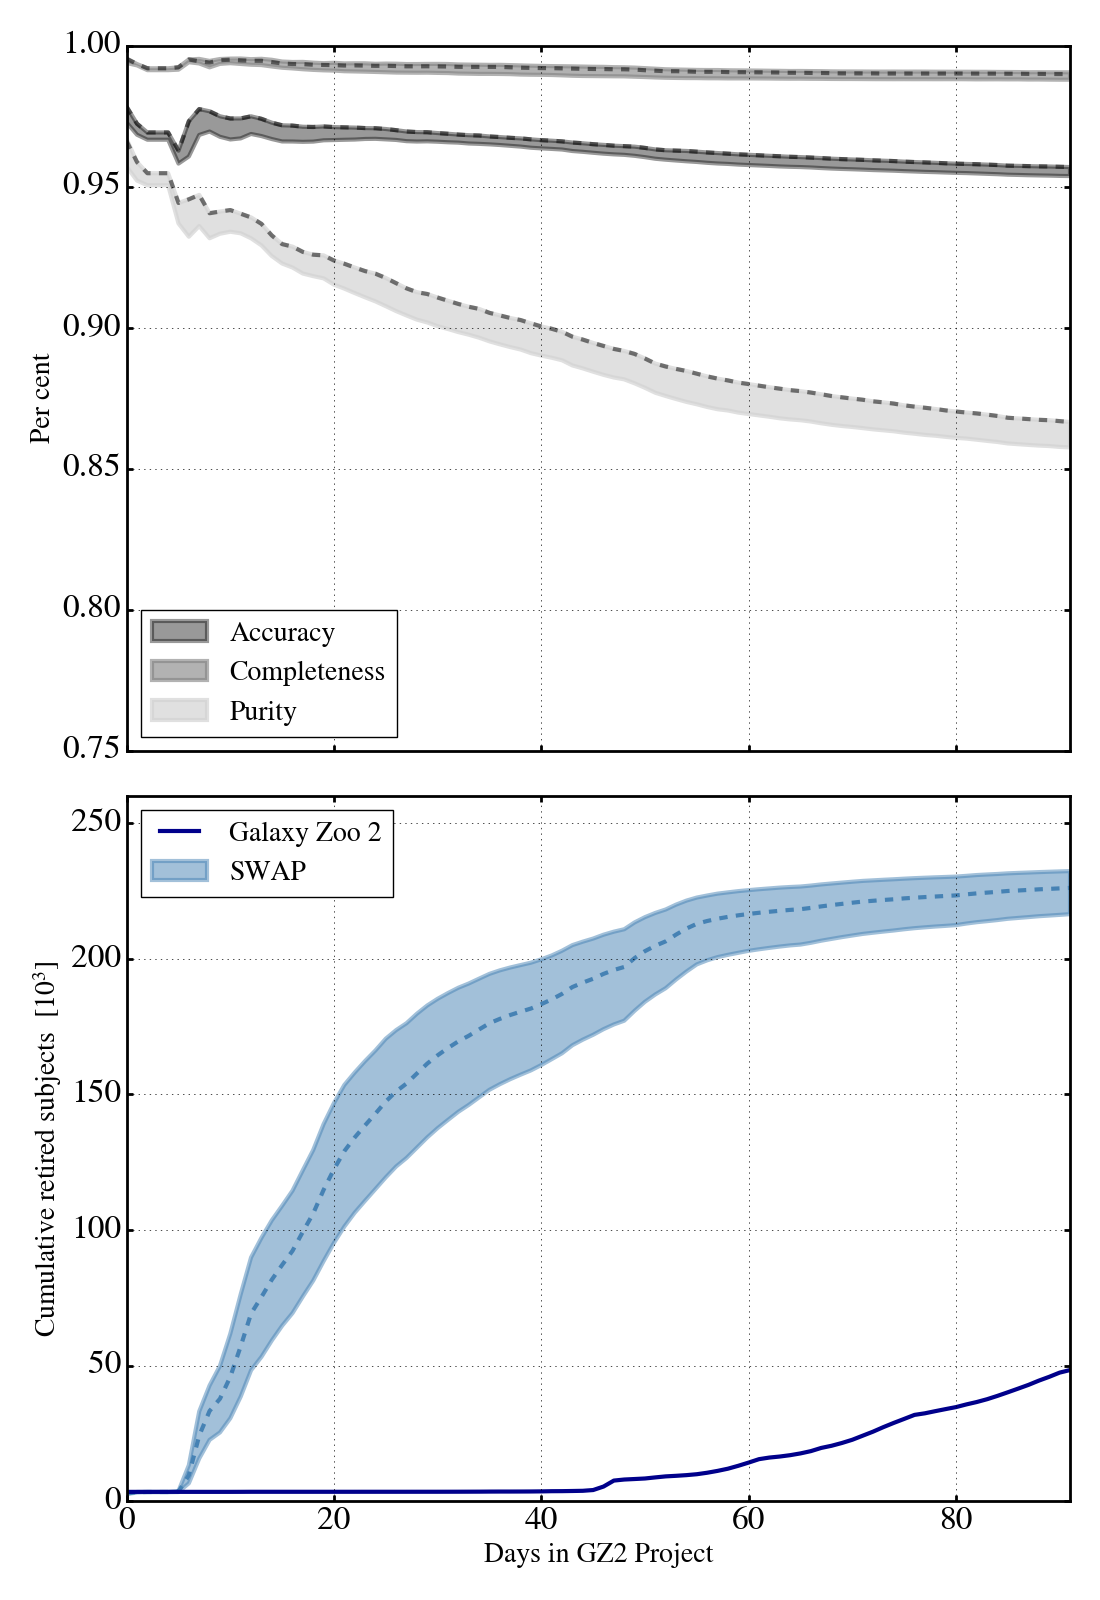
\includegraphics[width=3.5in]{figures/GZX_eval_and_retirement_PLPD_spread_4paper_v2.png}
\caption{GZX/SWAP output as a function of GZ2 project days for a range of initial
confusion matrix values.  \label{fig: confusionMatrixAnalysis}}
\end{figure}

\textbf{Initial agent confusion matrix.} 
In our fiducial simulation each volunteer was assigned an agent with confusion matrix
 (\Pf, \Pn) = $(0.5, 0.5)$, which presumes that volunteers are no better than 
random classifiers.  We perform two simulations wherein we allow (\Pf, \Pn) = $(0.4, 0.4)$, 
slightly obtuse volunteers, and (\Pf, \Pn) = $(0.6, 0.6)$, slightly astute volunteers 
with everything else remaining constant.  
Results of these simulations compared to the fiducial run are shown in 
Figure~\ref{fig: confusionMatrixAnalysis}. We find that we are largely insensitive to the 
initial agent confusion matrix probabilities both in terms of the overall number of retired subjects
and in the quality of their SWAP labels. 

Predictably, when (\Pf, \Pn) are low, we retire fewer subjects in the same time frame and 
more subjects when (\Pf, \Pn) are high. This is easy to understand since it takes 
longer for volunteers to become strong, astute classifiers when they are initially 
given values denoting them as obtuse. Even with this handicap, most volunteers 
become astute classifiers by the end of the simulation. Overall,  we retire 
$\sim225$K  $\pm 3.5\%$ subjects as shown by the light blue spread in the bottom
panel of Figure~\ref{fig: confusionMatrixAnalysis} where the dashed blue line
denotes the fiducial run. 

The top panel depicts the same quality metrics computed before where the dashed 
lines again denote the fiducial run.  The spread is within a couple per cent for any
metric. Overall we maintain accuracy around $95\%$, as well as completeness of $99\%$
while maintaining purity around $84\%$. This spread can be due to three different
effects: 1) classifying a different subset of subjects, 2) retiring subjects in a different
order, and 3) subjects acquiring a different SWAP label in different simulations. 

We find that SWAP is exceptionally consistent. Of all the subjects retired in
these runs, we find that over 99\% of them are the same subjects between simulations.
Of those consistent between runs, we find that SWAP gives the same label for 
more than 99\% of the subjects. What changes between runs is the order in 
which subjects are classified. In the low (\Pf, \Pn) run, subjects take longer to classify 
compared to the fiducial run (i.e., they retire on a later date in GZ2 project time). 
Subjects in the high (\Pf, \Pn) run retire earlier in GZ2 project time. This can cause
a variation in accuracy, completeness or purity because these values are 
calculated on a day to day basis; if we're working with a slightly different make-up
of subjects on a given day, we can expect to compute different values for these metrics.
These effects each contribute less than one per cent variation and thus we see a 
high level of consistency between these simulations. 



%% -------------------------------------------------------------------------------
%%   FIGURE:  SWAP -- vary SUBJECT PRIOR
%% -------------------------------------------------------------------------------
\begin{figure}[t!]
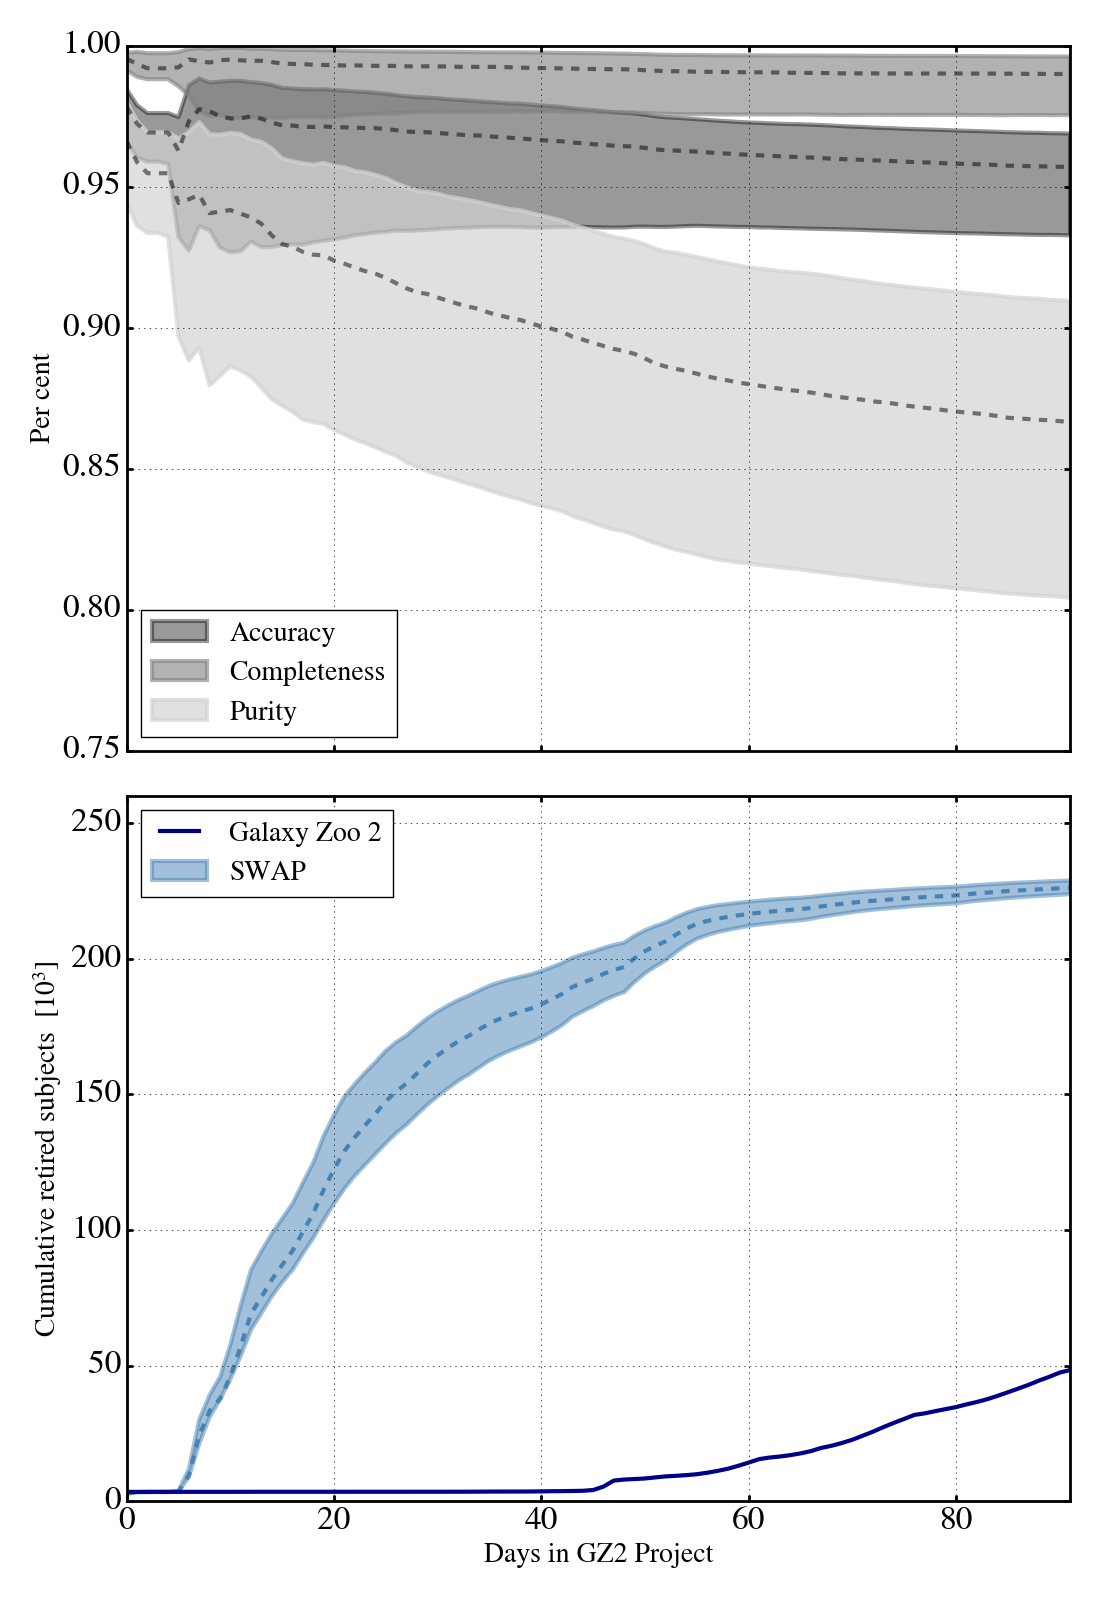
\includegraphics[width=3.5in]{figures/GZX_eval_and_retirement_prior_spread_4paper_v2.png}
\caption{GZX/SWAP output as a function of GZ2 project days for a range of subject prior probabilities.  \label{fig: priorAnalysis}}
\end{figure}


\textbf{Subject prior probability,~\p.}
The prior probability assigned to each subject is an educated guess of 
the frequency of that characteristic in the scope of the data at hand. 
For galaxy morphologies, this number should be an estimate of the probability
of observing a desired feature (bar, disk, ring, etc.). In our case, 
we desire to simply find galaxies that are~\feat, however, this is dependent 
on mass, redshift, physical size, etc. The original GZ2 sample was selected
primarily on magnitude and redshift.  As there was no cut on the galaxy size
(with the exception that each galaxy be larger than the SDSS PSF), the sample
includes a large range of galaxy masses and sizes. Thus, designating a single 
prior is not clear-cut. We thus explore how various~\p~affect the SWAP outcome.

We run several simulations where~\p~is allowed to take values 0.2, 0.35, and 0.8 
and compare these to the fiducial run where~\p~= 0.5, everything else remaining constant.
The results are shown in Figure~\ref{fig: priorAnalysis}, where again we find that 
SWAP is consistent in terms of the total number of subjects retired 
during the simulation which varies by only 1\%. 
However, as can be seen in the top panel, the variation in our quality metrics is 
more pronounced and deserves some discussion. 

Firstly, though we are retiring nearly the same number of subjects over the course
of each simulation, they are less consistent than our previous simulations. That is, 
only 95\% of the subjects are common to all runs. Secondly, of those that are 
common, only 94\% receive the same label from SWAP. Changing the prior is more
likely to produce a different label for a given subject than changing the initial 
agent confusion matrix. Finally, there is also a larger spread in the day on which 
a subject is retired when compared to the fiducial run, being nearly equally likely to 
retire `late' or `early' regardless of~\p. These trends all contribute to a broader 
spread in accuracy, completeness, and purity as a function of project time.
We stress, however, that though more substantial than the previous comparison, 
these variations are all within $\pm5\%$. 

We can get a handle on these variations more intuitively by considering the following.
Recall that our retirement thresholds,~\tf~and~\tn, have not changed in these simulations. 
Thus when~\p~is small, the subject probability is already closer to~\tn, and more 
subjects are classified as~\notfeat~compared to the fiducial run.
Similarly, when~\p~is large, some of these same subjects can instead be classified
as~\feat~because the prior probability is already closer to~\tf. Obviously, both 
outcomes cannot be correct and we find that the simulation with~\p~= 0.8 performs
the worst of any run which is a direct reflection of the fact that this prior is not 
suitable for this question nor for this dataset. For the mass, size, and redshift range
of subjects in GZ2, we would not expect that 80\% of them are~\feat. Indeed, 
the best performance is achieved when~\p = 0.35.  This reflects the actual 
distribution of~\feat~subjects in the GZ2 sample as well as being similar to the 
expected proportion of~\feat~galaxies in the local universe, depending on your
definition\textbf{ (cite studies of distribution of early and late type gals in local universe?). }
Thus, the take-away here is to choose your prior wisely since a value far from the correct
value can have a significant impact on the quality of your classifications.
 
%% -------------------------------------------------------------------------------
%%   FIGURE:  SWAP -- Retirement Thresholds
%% -------------------------------------------------------------------------------
\begin{figure}[t!]
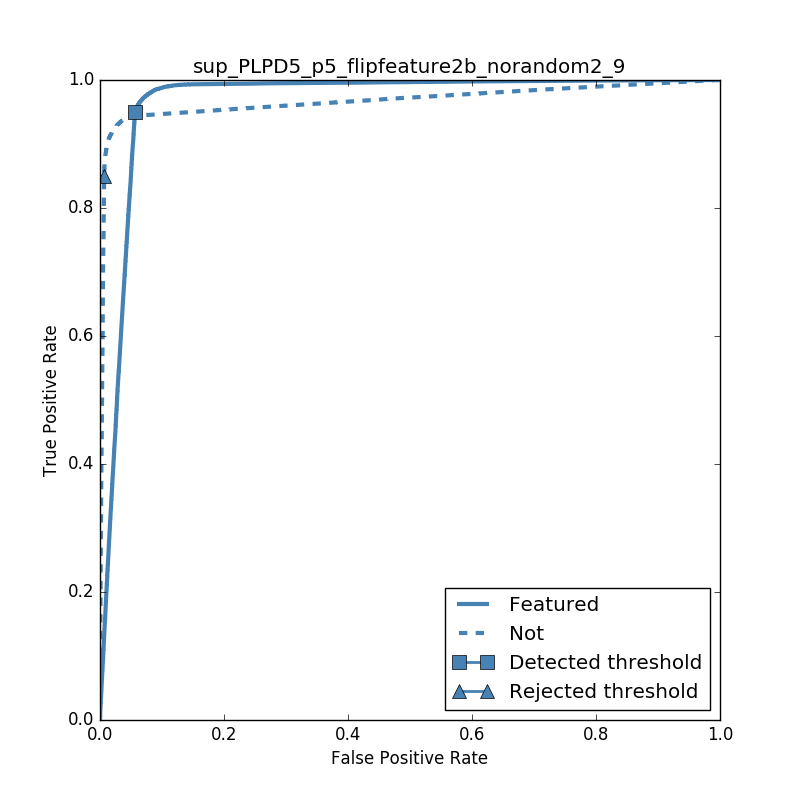
\includegraphics[width=3.5in]{figures/GZX_ROC_sup_PLPD5_p5_flipfeature2b_norandom2_9.png}
\caption{Retirement thresholds are adequate for our purposes.  \label{fig: retirement thresholds}}
\end{figure}


\textbf{Retirement thresholds.}
Retirement thresholds are directly related to the time that a subject will spend
in SWAP before retiring.  If we lower~\tf~(and/or raise~\tn), more subjects will be retired
compared to the fiducial run as each subject will have a smaller swath of probability space
in which to bounce back and forth before crossing one of these thresholds.
On the other hand, if we raise~\tf~(and/or lower~\tn), it will take longer for subjects
to cross one of these thresholds. Additionally, this will also increase the likelihood of
some subjects never crossing either threshold as there are always some 
which are nudged back and forth indefinitely through probability space.


What thresholds should one choose? To answer this question, we consider
Figure~\ref{fig: retirement thresholds} which depicts the receiver operating 
characteristic (ROC) curve for our fiducial simulation. The solid line shows the 
curve when considering the~\feat~threshold  while the dotted line
corresponds to~\notfeat. The square and triangle represent our thresholds, 
(\tf,~\tn) = (0.99, 0.004), on that curve at the end of the simulation.  We see that 
~\tf~is nearly optimal but~\tn~could be improved upon. 


Throughout this discussion we have computed quality metrics under the assumption
that the `true' labels provided by GZ2 are accurate. 
This is unlikely to be the case for every subject as~\cite{Willett2013} explicitly caution against using 
the majority volunteer vote fraction as label since some of these are highly uncertain. 
We now turn to a brief discussion of those subjects where SWAP and GZ2 do not agree. 



\subsection{Disagreements between SWAP and GZ2}

%%%-------------------------------------------------------
%%%  FIGURE:   SWAP failures
%%%-------------------------------------------------------
\begin{figure}[t!]
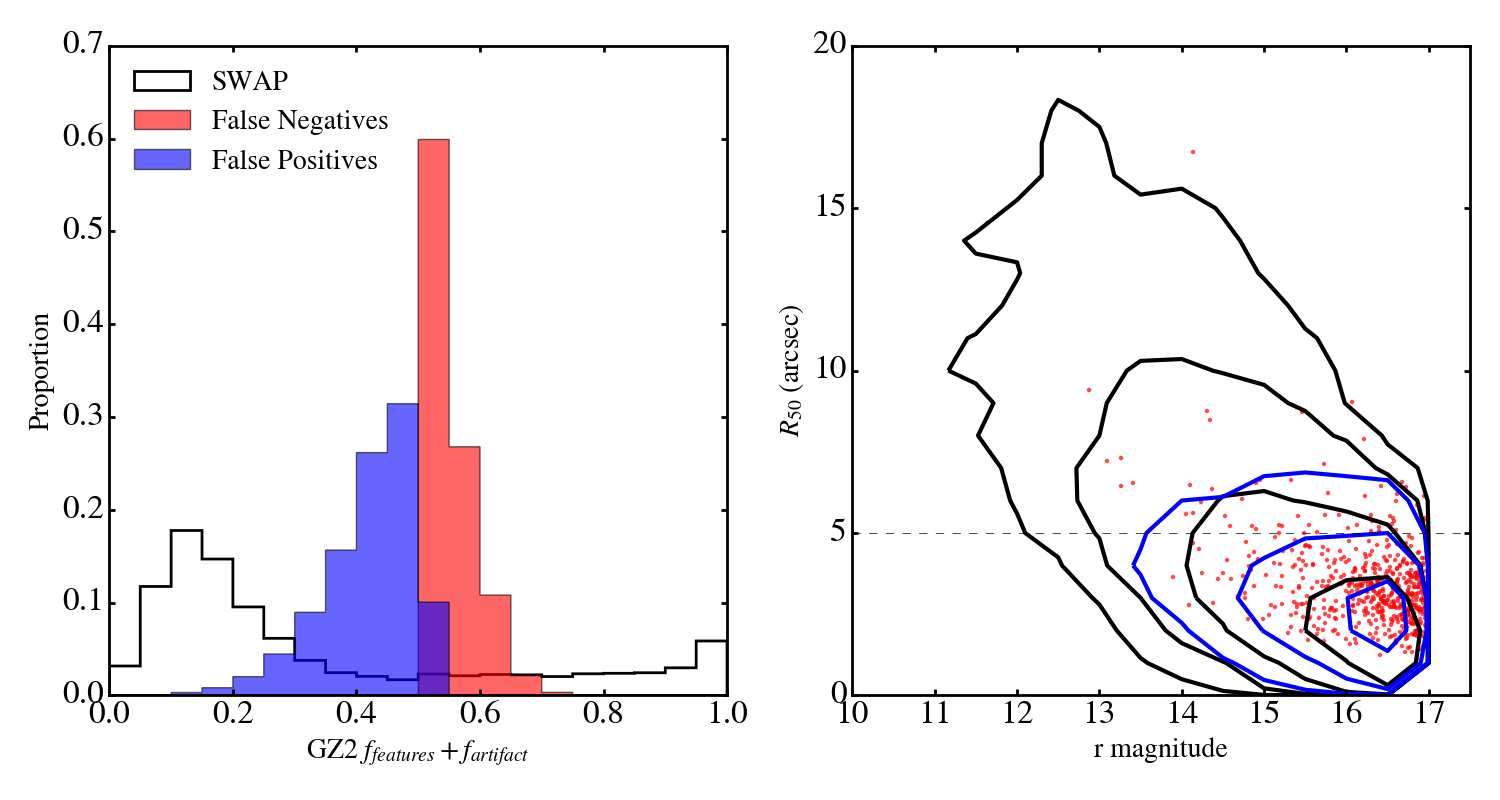
\includegraphics[width=3.65in]{figures/swapgetsitwrong_test.png}
\caption{SWAP and GZ2 labels disagree approximately 5\% of the time, depending on the choice
of initial SWAP parameters. The disagreement stems, in large part, from `true' labels derived from uncertain GZ2 vote fractions as shown in the left panel where the  majority of SWAP's false negative and false positive subjects have GZ2 vote fractions which fall in the range 0.4 - 0.6. Furthermore, it is unsurprising that these same subjects are physically more difficult to classify being, on average, smaller and fainter than the sample as a whole as shown in the right panel. \label{fig: SWAP sucks}}
\end{figure}

Galaxy Zoo's strength comes from the consensus of dozens of volunteers voting on each subject. 
Processing votes with SWAP effectively reduces this consensus to its bare minimum. 
Though we typically recover the GZ2 label, SWAP disagrees about 5\% of the time. 
In this section we examine the main effects driving this disagreement whereby we again
 turn to our fiducial simulation, isolating all false positives and false negatives. 

We find that the majority of these disagreements are due to uncertainties in the GZ2
label. This is shown in the left panel of Figure~\ref{fig: SWAP sucks} where we show
the distribution of the \texttt{features\_or\_disk} + \texttt{star\_or\_artifact} GZ2 vote 
fractions for the entire sample retired by SWAP (solid black lines). 
Recall that we group these together as~\feat~during  our SWAP simulations and so 
group them here for a fair comparison. Furthermore, because we used a majority vote
fraction to derive labels, any subject with $ f_{features}+f_{artifact} > 0.5$ would be
labeled~\feat.  However the false negative (red) distribution shows that a portion 
of these still attained a~\notfeat~label through SWAP (with the opposite being 
true for the blue false positive sample). In fact, the majority of incorrectly labeled 
subjects have $0.4 \le f_{features}+f_{artifact} \le 0.6$,
indicating that the GZ2 vote fractions are simply too uncertain to provide high quality labels. 

Another effect contributing to the disagreement is related but more subtle and 
concerns the order in which volunteers cast their votes. Consider a subject where
the first N volunteers classify it as X while the subsequent majority of volunteers classify
the subject as Y. Here the power of GZ2's large consensus shines because this lopsided 
voting is averaged out. SWAP, however, will swiftly kick that subject's probability 
over a retirement threshold when encountering such a chain of classifications. 
The result is SWAP labels which disagree with GZ2 labels purely due to order statistics. 
Consider a subject with a $f_{features}+f_{artifact} = 0.2$, where 40 unique volunteers have
classified this subject yielding a GZ2 label of~\notfeat. What is the probability that 
this subject will obtain a label~\feat~through SWAP? In other words, what is the 
probability that the first eight volunteers all voted~\feat?  If we assume all volunteers
have~\Pf~= 0.5, it is trivial to compute $1/2^8 = 0.39\%$. Of course, this effect is more
complicated to model in aggregate since volunteers have confusion matrices that vary 
with time and subjects can be retired with a varying amount of volunteer classifications. 

This leads to another subtle effect that can cause SWAP labels to disagree with GZ2 labels.
Volunteers generally do not have (\Pf,~\Pn) = (0.5, 0.5). We find that, occasionally, some 
subjects are retired with only two classifications because one of the volunteers had 
an exceptionally large confusion matrix. We estimate this effect at XXX. 

To prevent these issues, one could a.) require each volunteer classify a certain 
number of subjects to increase their confusion matrix values or
b.) require each subject reach a minimum number of classifications before allowing 
it's probability to cross a threshold. The difference lies between averaging over a 
volunteer's burn-in phase versus a subject's burn-in phase.
The latter is preferable as the majority of Zooniverse volunteers contribute only 
a small amount of classifications to any given project. Requiring they achieve a 
minimum classification count before allowing their contribution to count would 
hamstring the effectiveness of citizen science projects. 


\subsection{Summary}

We have demonstrated that, regardless of the initial configuration of the SWAP 
software, we achieve nearly an order of magnitude increase in the efficiency of 
classification corresponding to nearly an order of magnitude decrease in
required human effort. All of this can be obtained with sample accuracy over 95\%, 
almost perfect completeness of subjects designated as~\feat, and with a sample purity
that can be controlled by careful selection of input parameters to be better than 90\%. 
We've explored those subjects where the SWAP label and the GZ2 label disagree
and have shown that the majority of the disagreement lies in the uncertainty of 
our `true' labels with small contributions from idiosyncrasies in SWAP. 
Under this assumption, we now turn our focus towards incorporating machine
classifiers utilizing these SWAP-retired subjects as training samples. 


%%----------------------------------------------------------------------------------------------------------------------------------------------------
%%   INTEGRATING MACHINE CLASSIFIERS 
%%----------------------------------------------------------------------------------------------------------------------------------------------------
\section{Efficiency through incorporation of machine classifiers} \label{sec: machine}

In this section we construct the full Galaxy Zoo Express by incorporating supervised 
learning, the machine learning task of inference from labeled training data. 
The training data consist of a set of training examples, and must include
an input feature vector and a desired output label.  Generally speaking,
a supervised learning algorithm analyzes the training data and produces an inferred 
function that can then be mapped to new examples. An optimized algorithm will 
correctly determine class labels for unseen data. In general, most classification 
algorithms can handle prediction of several labels simultaneously. Work has been
done to predict the entirety of GZ2 classification labels using deep learning 
\citep{Dieleman2015} with great success. However, it is still simpler for a machine
to predict fewer labels than it is to predict several dozen, \textbf{[citation?]}, 
with the additional bonus that fewer class labels require less training data. 
By processing human classifications through SWAP we obtain a discrete, binary task
for a machine to tackle. We briefly outline the technical details of our machine
classifier before turning towards the decision engine we develop for GZX in 
section~\ref{sec: decision engine}. 


\subsection{Random Forests}
Because our task is simple, we choose a simple machine. In particular, we use 
a Random Forest (RF) algorithm,  an ensemble classifier that operates by bootstrapping
the training data and constructing a multitude of individual decision tree algorithms, 
one for each subsample.  An individual decision tree works by deciding which of 
the input features best separates the classes. It does this by performing 
splits on the values of the input feature that minimize the classification 
error. These feature splits proceed recursively. As such, decision trees alone are
 prone to overfitting the training data thus precluding them from generalizing 
well to new data. Random Forests mitigate this effect by combining the 
output label from a multitude of decision trees.  In particular we use the 
\texttt{RandomForestClassifier} from the Python module \texttt{scikit-learn}
\citep{scikit-learn}. 

\begin{comment}
%One of the simplest algorithms to conceptualize and use is the K-nearest neighbors (KNN) classifier. This classifier works simply by considering the K neighbors nearest to the test point in Euclidean space. As we have only a binary classification challenge, the test point is classified according to the majority of its K neighbors. In the event of a tie, the label if the closest neighbor to the test point determines its class. Though simplistic, this algorithm is surprisingly powerful in that it performs well in higher-dimensional space and is relatively fast to train. Obviously, the most important parameter to consider is the number of nearest neighbors to assign to each test point. But this is pretty much the only knob to turn in this method which is another benefit -- ease of interpretation. 
%We use scikit-learn's implementation of K-Nearest Neighbor Classifier (KNC) and optimize the K parameter. 
\end{comment}


\subsection{Cross-validation}
Of fundamental importance is the task of choosing an algorithm's hyperparameters, 
values which determine how the machine learns.  In the case of a RF, one must 
choose the maximum depth of the tree, the minimum leaf size, the maximum
number of leaf nodes, etc. The goal is to determine which values will optimize 
the machine's performance and thus cannot be choosen \textit{a priori}. 
Idealy, one would train the machine with every combination of parameters and 
consider the resulting performance by testing the trained machine on a sample
withheld from the training sample so as not to contaminate the results. 
Formally, we perform k-fold cross-validation whereby the training sample is split
into $k$ subsamples. One such subsample is withheld while the remaining data is
used to train the machine. This is performed $k$ times and the average performance
value is recorded. The entire process is repeated for every combination of the 
specified hyperparameter space and values that optimize the output are choosen. 

 
\subsection{Feature Representation and Pre-Processing}
Machine learning algorithms require a feature vector for each training example. 
This vector is composed of D individual numeric quantities associated with the 
subject which the machine will use to discern that subject from others in the 
training sample. To segregate~\feat~from~\notfeat~our feature set draws 
on ZEST \citep{Scarlata2007} and  is composed of Concentration, Asymmetry, Gini, 
M$_{20}$ and Source Extractor's ellipticity 
(See Appendix \ref{sec:Appendix} for details concerning the measurement process). 
These non-parametric indicators have long been used to 
quantify galaxy morphology in an automated fashion \textbf{citations: Conselice? Peth? Huertas-company?}. 
Altogether, these features describe a five dimensional parameter space in 
which the machine attempts to distinguish between the two classes. 
As the RF algorithm is capabale of handling high-dimensional parameter spaces, in
a future paper we will explore increasing our feature space to include parametric
morphology indicators such as Sersic index and B/T ratio. 

Another benefit of the RF algorithm is the flexibility with which it can accept input 
features. Most algorithms require that feature vectors be processed suth that all 
dimensions lie on the same scale. This is not necessary with an RF. The only
preprocessing required in our case is the removal of morphological paramters which
were not well-measured, i.e. catastrophic failures. 

%\textbf{Should this paragraph be here? Probably not. But it should be somewhere?}
%This is quite distinct from \textit{deep learning} methods which can learn on every 
%pixel of an image through a series of non-linear transformations. This technique has
%been successful at predicting galaxy morphology labels as explored by 
%\cite{Huertas-Company2015}, \cite{Dieleman2015} and others. In this work our focus
%is to outline a practical method to efficiently combine human and machine classification,
%not seek the most optimal or accurate machine algorithm. We are concerned more 
%with speed and simplicity though we stress that a machine is just an algorithm. 
%In the future, this particular application will accommodate any algorithm, including 
%deep learning techniques, should they so be desired. 

%Though deep learning methods promise new heights of classification accuracy, there are some drawbacks. Most notably, the interpration of these methods in the context of physical quantities is lacking. Because of the complex suite of layered non-linear transformations, it is difficult to backstrapolate what qualities of the image were most successful at understanding that galaxy's morphology. Moreover, connecting that to physical mechanisms within the galaxy remains to be seen. On the other hand, much work has been invested in connecting aggregate features such as CAS, G-M20 which are well demonstrated to correlate with specific galaxy stuffs like SFH and ... whatnots.. and described below.


%Before we feed the algorithm with these feature vectors we first perform two pre-processing steps. First, we clean the data as there are some very few number of cases where our algorithm failed to recover appropriate values for the Petrosian radius, C, A, G, or M20. Our code represents these failures as infs or nans and we thus remove these subjects from all samples.  The second transformation puts each of the features on equal footing. Taken at face value, each of the five morphology parameters resides in a different range of values:  M20 is nearly always negative as it is logarithmic, while Asymmetry and Gini are always between 0 and 1.  In order for the machine classifier to treat all features equally we scale each feature along columns. If a row represents an individual subject, then a column represents the same feature for all subjects. We normalize each subject's features in the standard way: 
\begin{comment}
\begin{equation}
z_{feature} = \frac{f_i - \mu}{\sigma}
\end{equation} 
Where $f_i$ is the $i$th subject's feature value, $\mu$ is the mean of the entire feature sample, and $\sigma$ is the standard deviation of the entire feature sample. This scales each feature to values between 0 and 1. 
\end{comment}


\subsection{Training and Validation Samples}
We are now ready to discuss the training sample in more detail. As we showed in the previous 
section, SWAP retires subjects far more rapidly than GZ2
by adaptively tracking volunteer skill and subject probabilities in a Bayesian framework.
This provides us with a way of quickly generating large subject samples with accurate
labels provided by human classifications that are dynamically generated as a function
of GZ2 project time. For the following analysis we again build
off of our fiducial model where, according to Figure~\ref{fig: fiducial run},
SWAP retires XXX subjects within 10 days. 

As discussed above, in addition to a training sample we also desire a validation 
sample to estimate the generalization (true) error of our trained machine. For 
this purpose we maximize the utility of our expertly classified sample. This sample
thus provides training to our volunteers and verification for our machine. 

\subsection{Decision Engine}\label{sec: decision engine}
A number of decisions must be made before attempting to train the machine. 
Which SWAP subjects should be designated as the training sample? 
When should we attempt the first training session? 
How do we decide when the machine has successfully trained enough to be
applied to unseen subjects? These are the core issues that we address
in our machine learning decision engine.

\textbf{Which subjects should provide the training sample?} As mentioned above, SWAP
yields a probability that a subject exhibits the feature of choice. A RF requires a
distinct label so we use only those subjects which have crossed either of the 
retirement thresholds. However, subjects do not cross these thresholds with equal rates. 
At any given stage in the simulation, the ratio of retired~\feat~to~\notfeat~is not
guaranteed to be balanced, thus yielding an unbalanced training sample.
 However, as a first test, we allow the machine to learn on all high probability subjects. 

\textbf{When should we attempt the first training session?}
During the couple days of the simulation, SWAP retires a few hundred subjects.
One could, in principle, train a machine with such a small sample, but the resulting
predictions on the test sample will be exceptionally poor. Furthermore, the machine
won't know that it's performing poorly. For example, if a training sample consists of
100~\feat~subjects, the machine will subsequently predict that every member of the 
test sample is also~\feat~with high probability. This is obviously wrong. 
In practice, a much larger training size is required for the machine to learn the 
true parameter space in which the feature vectors reside, but there is no hard rule
for choosing this number. Because RF is a simple model, we initially require that 
the training sample consist of at least 10K subjects before attempting the first training session. 

\textbf{When has the machine trained enough?} 
We assess our machine's learning status by first considering a learning curve, 
an illustration of a model's performance with increasing sample size for fixed 
model complexity. An example is shown in \textbf{Fig XXX} 
for a RF with fixed hyperparameters. The cross-validation score is the accuracy
resulting from k-fold cross-validation. The training score is the resulting machine
applied to the training sample. When the sample size is small, the cross-validation
score is low while the training score is high. This is a clear demonstration of a model
overfitting the data. As the training sample size 
increases, the cross-validation score increases while the training score decreases. 
Eventually both plateau, regardless of how large the training sample grows. 
This demonstrates that, after a certain point, for a fixed complexity model, 
larger training sets yield little additional gain. That the training
score reduces almost to the cross-validation score signifies that this particular
model is not well suited to capturing the complexity of the data set. 
A more sophisticated model would, in turn, likely require a larger training
sample. 

We use this general feature of any machine learning process to guide our 
decision making. We cannot reproduce a true learning curve
because the cross-validation procedure we perform can, in principle and in practice, 
yield a different set of machine hyperparameters that are most appropriate
for the training sample it received that night.  Instead, we look for the characteristic 
cross-validation score plateau. At each timestep, our software keeps record of 
the machine's training performance, including how well it scores on the 
training sample (to estimate overfitting), cross-validation score, 
and the best hyperparameters. When the machine's 
cross-validations score remains within 1\% on three consecutive nights, 
we deem the machine's performance acceptable. 


\subsection{The Machine Shop}
We can now describe a full GZX simulation. A typical run begins with human classifications 
processed through SWAP for several days. During that time, humans `train' on the 
gold standard sample and then begin classifying the main sample.  Once they retire 
at least 10K subjects, these are passed to the machine which trains for the first time. 
A suite of performance metrics are recorded by a machine \textit{agent}, similar
in construction to SWAP's \textit{agents}. Each night, the machine agent determines 
whether or not the machine has sufficiently trained by assessing all previous nights of 
training, comparing the variation in performance metrics. Once the machine has
passed the criterion laid out above, the agent introduces the machine to the test sample
which consists of any subject that has not yet been seen by humans, has not yet 
reached retirement through SWAP, has not been previously classified by itself, 
and is not part of the gold standard sample.  

What constitutes a machine classification? Once the trained machine is applied to
the test sample it will provide predictions for every subject therein, but these predictions
are not made with the same certainty. Most machine algorithms allow one to obtain
a probability associated with each subject's predicted label. 
In the case of an RF, this probability is simply the average of the probabilities of each 
individual decision tree where the probability of a single tree is determined as the fraction
of subjects of class X on a leaf node.  We use this probability to assess subjects about which
the machine is most confident (though we note it is not a true measure of confidence).
Only subjects that receive a class prediction with $p_{machine} \ge 0.9$ are considered
retired and hence removed from the system. The remaining subjects have the possibility 
of being classified by humans (or the machine again) during future timesteps. 


This is the embodiment of our feedback loop. Those subjects on which the machine
is least confident can be examined by human classifiers, potentially becoming part of the
training sample during a future cycle. Ideally, this increased training sample will 
cover a larger portion of the parameter space in which the machine can learn. 
With additional subjects spanning all of the parameter space, 
the machine can quickly achieve its maximum performance. 

In the future we will create a more sophisticated feedback mechanism whereby we 
can send particularly challenging subjects to super-users for identification (where 
these users can be identified by their high confusion matrix values as determined by SWAP,
 see section~\ref{sec: SWAP}). Additionally we can perform periodic spot-checks 
to confirm the machine's performance by cross-checking with humans for label consistency. 


\begin{comment}
In figure \ref{fig:testmetrics},
we can see how the machine is performing on the test sample as a function of 
project time. Understandably, the performance is poor the first time the machine 
crosses the `learnned` criterion. Flukes can happen and it was most likely not
quite as learned as expected or desired. However, as the project progresses the 
performance on the test sample increases. In particular, the black line denotes 
the performance as obtained on the entire test sample and we can see that even 
when the machine is at its peak, the accuracy doesn't increase much beyond 70\%. 
The red line, however, is when we select only those subjects which the machine is
most confident about (more than 90\% confidence, in particular). Now the accuracy
of the machine on this subsample reaches nearly 85\%.  

This allows us to set a criterion for which subjects the machine should be allowed
to retire from the system. We don't necessarily trust it on all subjects but can we 
trust it when it's most confident? Explore this more? 

Our system has now incorporated both clever use of human classifications and 
integrated machine classification. We now simulate the final element which is the
feedback mechanism. Those subjects which the machine is most confident about are 
flagged as retired and votes on these subjects are no longer recorded in SWAP or 
elseware. Those which the machine is not confident, however, remain in the pool 
such that, during the next timestep, volunteers can contribute to the classification 
of that subject. This will increase the diversity of the training sample thus 
providing the machine with a larger sample space in which to learn. 
\end{comment}

%%----------------------------------------------------------------------------------------------------------------------------------------------------
%%   RESULTS 
%%----------------------------------------------------------------------------------------------------------------------------------------------------
\section{Results} \label{sec: results}
We perform a full GZX simulation incorporating both SWAP and our RF machine using the
 fiducial SWAP run discussed in section~\ref{sec: fiducial}. 
The machine attempts its first training on Day 8 of the run with an initial training
sample of nearly 20K subjects.  The machine undergoes several additional nights of training, 
each time with a larger training sample. 
By Day 12, the machine's \textit{agent} has assessed that the machine is suitably trained. 
At this point, SWAP has now provided over 40K subjects as a training sample. 
The machine predicts class labels for the remaining 230K GZ2 subjects which are not 
already retired by SWAP or part of the expertly classified sample. 
Of those, the machine strongly predicts labels ($p_{machine} >= 0.9$ for nearly 71K subjects, 
thus immediately and dramatically increasing the overall sample of retired subjects. 
As the simulation progresses, retirement by both SWAP and
the machine tapers off though at different rates. 
We end the simulation after 32 days, having sufficiently classified well over 200K subjects. 
We present these results in the bottom panel of Figure~\ref{fig: money} where GZX (red) 
is compared to our fiducial SWAP only run (light blue) and GZ2 subject retirement (dark blue). 

%%%-------------------------------------------------------
%%%  FIGURE:    FULL GZX PERFORMANCE
%%%-------------------------------------------------------
\begin{figure}[t!]
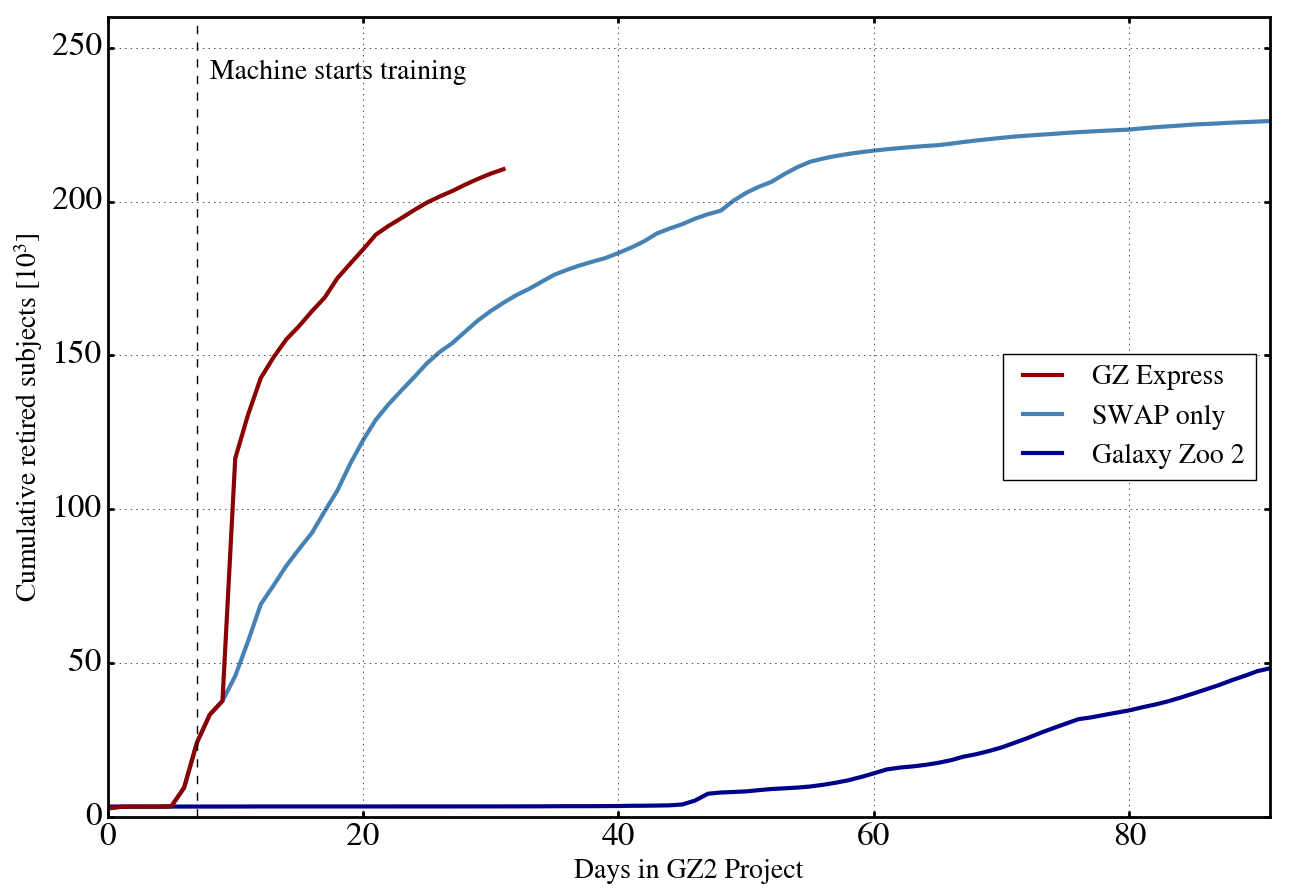
\includegraphics[width=3.65in]{figures/GZ2_sup_PLPD5_p5_flipfeature2b_RF_accuracy_redo_raw_combo_moneyplot.png}
\caption{Incorporating the machine reduces the total time to classify over 200K subjects in the GZ2 sample to 23 days. \label{fig: money}}
\end{figure}

The top panel of Figure~\ref{fig: money} shows our usual quality metrics for both 
SWAP-only and GZX, again using the GZ2 labels discussed in section~\ref{sec: data}.
Accuracy and completeness of the cumulative sample for the combined system 
each remain around 95\% and purity remains around 85\%. We note that 
incorporating the machine yields similar purity as when we 
allow SWAP to handle the entirety of the sample for a similar-sized subject set. 
Instead we seem to make a small sacrifice in the completeness of the~\feat~sample
which, in turn, affects our accuracy. Whereas SWAP alone identifies nearly all~\feat~
subjects it encounters,  the machine appears to miss a significant 
portion of these thus dropping the completeness of that day's 
cumulative sample. We discuss this behavior below.

By dynamically generating a training sample
through a more sophisticated analysis of human classifications coupled with a 
machine classifier trained through a simple feedback mechanism, we are able to 
retire over 200K GZ2 subjects in 27 days.  SWAP alone retires as many subjects in 50 days
while GZ2 requires XX \textit{months} to retire as many and 14 months to retire 
the entire catalog of 285K subjects. 
GZX thus provides \textit{a full order of magnitude decrease in classification time} 
over the traditional crowd-sourced approach. 
We next explore the composition of those classifications.


\subsection{Who retires what, when?}  

%%%-------------------------------------------------------
%%%  FIGURE:    GZX COMPONENT CONTRIBUTIONS
%%%-------------------------------------------------------
\begin{figure}[t!]
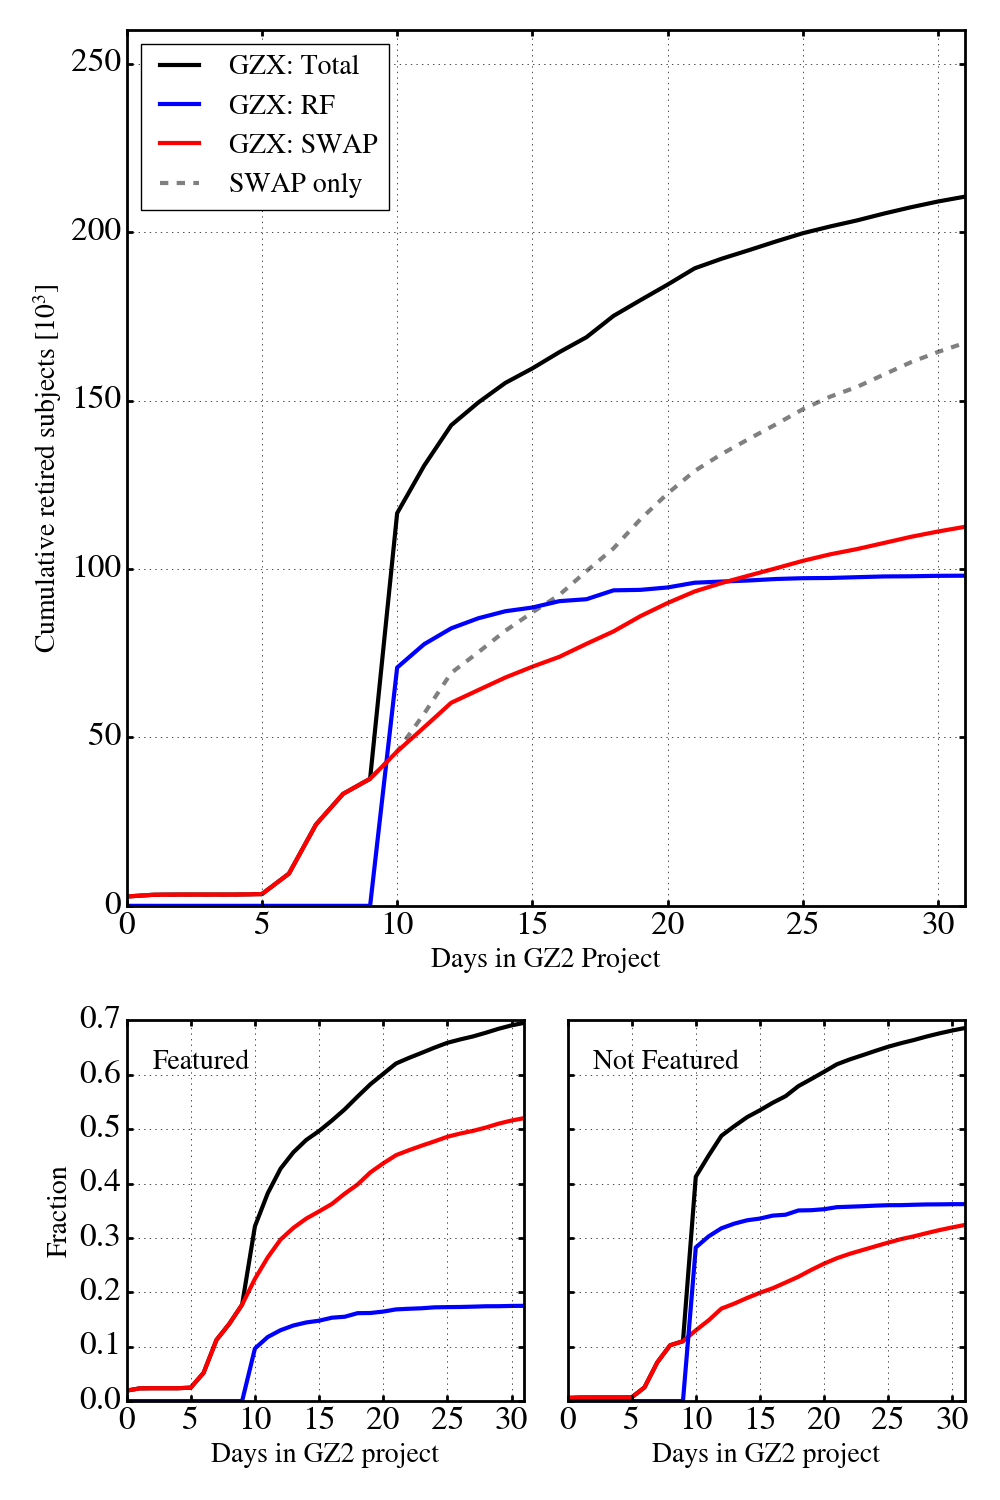
\includegraphics[width=3.65in]{figures/GZ2_sup_PLPD5_p5_flipfeature2b_RF_accuracy_redo_raw_combo_GZX_component_contributions.png}
\caption{The relative contributions of the human and machine components of GZX are nearly equal but display very different behaviors over the course of our simulation.  \label{fig: gzx components}}
\end{figure}

In Figure~\ref{fig: gzx components} we explore the relative contribution from both the 
machine (blue) and SWAP (red). The solid black line shows the full GZX retirement 
and the dashed line shows the SWAP-only fiducial run from section~\ref{sec: fiducial}. 
Two things are immediately obvious. 
First, we see that, over the course of our simulation, the machine retires a total of 
$\sim100$K subjects while SWAP retires $\sim110$K subjects. Each shoulders approximately
half of the classification burden. Secondly, the behavior in the rates of these
retirements is clearly very different. Retirement through SWAP proceeds at a relatively
constant rate from Days 5 through 25 before beginning to taper off. In contrast, 
the machine contributes a massive surge in retirement during its first couple days 
quickly overtaking the human contribution but plateaus dramatically thereafter.
By Day 22, the human contribution through SWAP  again becomes the primary mode 
of subject retirement. 

Thus we clearly see  three epochs of subject retirement, as we presumed.
In the first phase humans are the only contributors to the total number of retired subjects.  
Once the machine has trained, it becomes a workhorse and takes a monstrous share 
of the retirement burden though humans also contribute. 
The machine quickly reaches it's peak performance, classifying all subjects 
it's capable of recognizing and the third phase is thus left to humans who again dominate 
the the rate of subject retirement. 

Finally, we consider the composition of the two classifying agents. 
Throughout the simulation, SWAP consistently retires, 38\% to 40\% of subjects
 as~\feat~on any given night of the run. 
In contrast, the machine labels only 14\% of retired subjects as~\feat~the first 
night it runs and only 20\% are labeled~\feat~by the last day of the simulation. 
Of all retired subjects, 27\% of them have a~\feat~label according to their majority
 GZ2 raw vote fractions. This suggests that humans are more likely to identify
obviously~\feat~galaxies while the machine seems predisposed to identify the converse.
That humans and machine might be optimized  somewhat divergently is not surprising when 
one considers that they are presented with different information and learn in 
entirely distinct ways.  In the next section we explore  the machine's classifications 
in more detail to understand the core of its performance.


\subsection{Machine-only performance}
The results presented above considered all subjects retired by the combined GZX system:
machine and humans. We now look specifically at the machine's contribution. 

When considering the machine's performance alone, we turn to figure
~\ref{fig: machine accuracy} which shows the accuracy of the machine-retired
 (high probability) subjects in red along with the number of machine-retired subjects (black). 
We see that the first application yields exceptionally good accuracy considering
the machine of choice. However, this accuracy of drops to 75\% by the end of the simulation.
We note also that the machine retires X times more subjects on its first 
application to the test sample but never again retires as many on subsequent nights. 
Of those it does retire, the machine predominately classifies~\notfeat~(`Smooth') subjects
far better both in terms of the number it can classify and in the quality of those classifications. 
These are obvious symptoms of an unbalanced sample. 


We're comparing all output to the GZ2 raw vote frations because we find that this is 
the best choice for fair comparisons with SWAP output. However, the machine is different.
It is presented with different information and learns a different way which can result in 
a very differnet answer. We thus carefully reconsider what constitutes the truth label to
which we should ultimately compare the machine's output. 

The machine is trained with labels provided by SWAP for which we find the best comparison 
is the GZ2 raw vote fraction discussed earlier. However, does it make sense 
for the machine to provide those labels given the input it receives? It has a 5 dimensional 
morphology parameter space to explore which is very different from the much higher
dimensional space of a color jpeg that the humans see. However, these parameters are
specifically known to correlate with various galaxy morphology properties in a more or less
predictable way. For example, galaxies with very high ellipticity are predominantly 
edge-on galaxies and would thus fall under the~\feat~category while galaxies with 
high concentrations would suggest a smooth or~\notfeat~subject. 
The question becomes: What exactly has the machine learned? And what labels are 
most appropriate to compare what it's learned to asldfkjsldfjasd. 
 
The quality metrics for the GZX in figure~\ref{fig: money} were computed using the 
GZ2 raw vote fractions. 


Separate what is particular to THIS MACHINE versus what is generalizable to ALL MACHINES.

ALL Machines: 1. unbalanced sample will make classification difficult, 2. we're comparing labels
that aren't necessarily apples to apples because we're asking the machine \textbf{a different question with different data!} 3. Not necessarily true that the set of 

THIS Machine: 1. is particularly terrible at spotting \feat~ for some reason

We now turn to a discussion of what subjects can and can't be classified and why. 
We argue that our method provides a quick way to determine which subjects will
inevitably be suitable for either visual or machine classification and which subjects
simply provide too little information for robust classification. This knowledge, coupled
with the fast classification rate will enable large scale surveys to efficiently and effectively
tackle morphological classification tasks. 


\begin{comment}
%%%-------------------------------------------------------
%%%  FIGURE:    Machine Accuracy
%%%-------------------------------------------------------
\begin{figure}[t!]
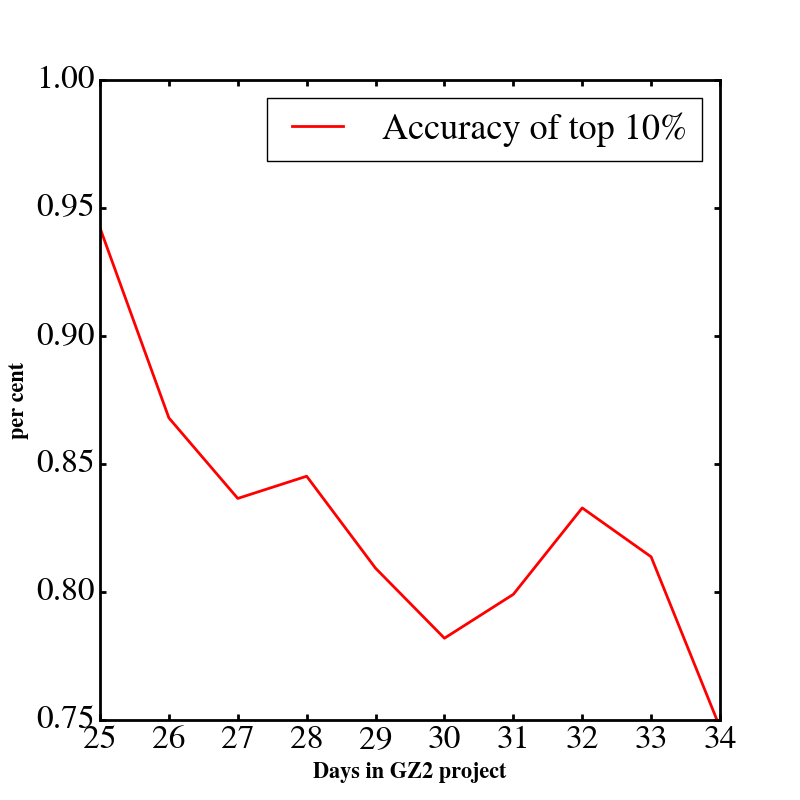
\includegraphics[width=3.65in]{figures/MLevaluation_GZ2_sup_PLPD5_p5_flipfeature2b_RF_accuracy.png}
\caption{Incorporating the machine reduces the total time to classify over 200K subjects in the GZ2 sample to 23 days. \label{fig: machine accuracy}}
\end{figure}
\end{comment}

\begin{comment}
%We examine in the size-magnitude plane those  subjects retired by machine as shown in Fig~\ref{fig: machine classified}.  We see see the first classification by the machine includes a healthy mix of both `Featured` and `Not' subjects over a broad range of magnitude and sizes. These subjects are "easy to classify" as they are large and bright. However, by the end of the run the machine (combined with SWAP) have classifed the easiest subjects; those with the most information stored in their images.  On the last day we peform the simulation, the machine is only classifying small, faint  subjects; all the larger and brighter subjects have been retired. Small, faint subjects are notoriously difficult to classify. As such, when comparing the resulting prediction from the machine to the original label provided by GZ2, it is less likely that machine matches that prediction. Indeed, it is just as likely that the original GZ2 classifications are inherently wrong themselves. \textbf{Show a random sample of original jpg images? } 
\end{comment}

This trend can even be seen in the SWAP-only output. 
Fig~\ref{fig: swap} shows the accuracy of the SWAP output slowly decreases 
over the life of the project coupled with the strong tapering of classifications 
are both sure signs that the easiest to classify galaxies have been retired leaving
more difficult, if even classifiable, subjects in the queue. 

%%%-------------------------------------------------------
%%%  FIGURE:    Machine classifies SHITTIER SUBJECTS -- OR DOES IT? 
%%%-------------------------------------------------------
\begin{figure*}[t!]
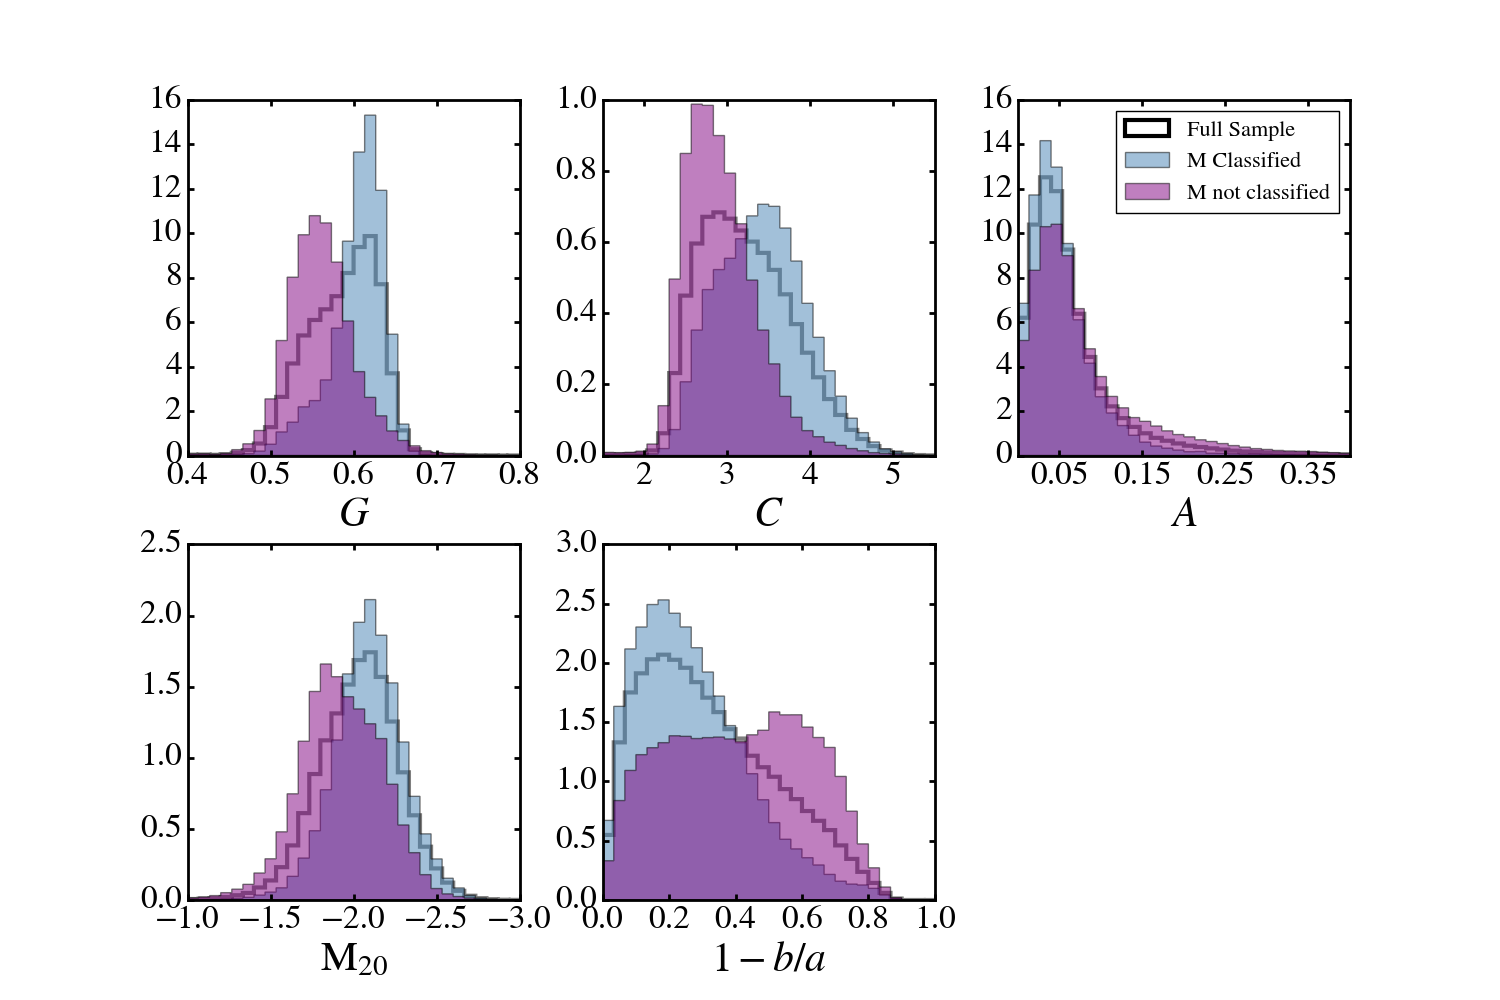
\includegraphics[width=7in]{figures/machine_compare_clssfd_not_morph_params1D.png}
\caption{What the machine can and can't classify. \label{fig: machine classified}}
\end{figure*}

We also examine those subjects which are not classified at all, either in the SWAP-only
run or the combine run. I am sure they will all suck but need to throw up some distributions
REDSHIFT, MAGNITUDE, SIZE.  Indeed, the original GZ2classifications were never intended 
to be used directly as a catalog. The authors strongly urge cuts down the decision tree as
as well as in magnitude and redshift. Even the power of human consensus  cannot 
classify information which is not provided by an image. \textbf{The third way we increase 
efficiency is to effectively identify those subjects for which additional human or 
machine intervention is not practical and will not yield appropriate classifications.} 




%%----------------------------------------------------------------------------------------------------------------------------------------------------
%%   MAD RAVINGS OF THE FUTURE 
%%----------------------------------------------------------------------------------------------------------------------------------------------------
\section{Implications and Recommendations}\label{sec: visions}

We've now identified several ways to suss out those subjects which require
additional intervention. If SWAP can't classify it, then potentially these subjects 
should be diverted to experts. If a machine can't classify it, then those subjects
can be relegated back to humans. Thus we have a cute little chain of command!

Apply all these performance metrics to the datasets expected from Euclid, LSST, etc. 
Estimate reduction in classification time. 

\subsection{Short-term Visions}

Immediate steps we can take to make a stronger system.

1. more sophistcated feedback mechanism

2. more sophisticated machine (deep learning? LDA? )

3. larger feature vector

4. ultimate ensemble classifiers where machine votes are processed through their own instance of SWAP!

5. SWAP that allows for a 3-way confusion matrix


\textbf{Classifications are not debiased.}  
It is a known issue that any visual 
classification will be biased by several effects, especially redshift and size. 
Lack of depth and resolution at higher redshift tend to produce classifications 
which lack observable features. Galaxy Zoo 2 is able to account for redshift bias
by adjusting the vote fractions produced by the volunteers. This step is done after
the fact by considering for every Galaxy Zoo catalog
 \cite{Willett2013}, \cite{Willett2016}, \cite{Simmons2016}. 
Throughout this paper, we compare predicted classes to a majority raw GZ2 vote fractions.
These vote fractions are not corrected for redshift bias. As states above, we chose
these vote fractions because SWAP processes the original votes and does not 
have functionality to debias these votes. Thus, this step must still be done 
after subjects are retired or the project completes. 


\textbf{Where does the gold standard sample come from?}
Of utmost importance to GZX is the establishment of a gold standard sample. 
We utilized this sample both to provide "training" for volunteers and to provide 
validation for the machine. Applications of GZX to other surveys and projects will
require PIs to develop appropriate gold standard samples of their own data. 
How should these samples be developed?
How should the labels be applied? Luckily, the Zooniverse Project Builder is an 
open source, free to use, web based service which allows teams to build and classify
their own data.
 How large should the sample be?  Unfortunately, it is outside the scope of this paper
to produce a larger gold standard sample for testing purposes. However, we have 
unequivocally demonstrated that with a sample of ~3500 subjects, we are able to 
achieve adequate results. 
\textbf{It would be soooo cool to run SWAP again with fewer gold standard subjects; 
or play around with how the classifications on gold standard subjects are distributed throughout the data. :(}


\textbf{We didn't actually train volunteers.}
The Space Warps project provided feedback to volunteers after their classification
of simulated data thus providing practical training for their volunteers. We stress 
that, although we have strived to mimic this process, we are reprocessing data and
thus could not provide feedback in real time. The extent of this effect outside the scope
of this paper, however, results of an application of SWAP to a live project 
are explored in Wright2016, in prep \ref{Wright2016}. 
\textbf{Notes: Fewer users trained. Fewer training images. 
Less front-loading (how far apart can the training images be staggered and still produce good results?)}


\textbf{Low redshift regime -- what can we do for higher z data?}
GZ2 is a low redshift sample of galaxies, those to which the Hubble tuning fork 
could be applied. At higher redshift, these class labels break down. 
Similarly, standard methods of quantifying morphological structure also 
suffer as M20 and Gini coefficient are susceptible to noise (I think, cite XXX).
Additionally, as the shapes of galaxies are significantly different at higher 
redshift, different metrics of morphology would be more appropriate. 
We could easily extend our machine to perform on high redshift samples
by incorporating the MID statistics \ref{Freedman2013}. Another future
test will be to examine how GZX performs on Galaxy Zoo: Hubble and 
Galaxy Zoo: CANDELS datasets. 

\textbf{Naive machinery -- RF is too simplistic}
Fig~\ref{fig: machine too simple} shows the pseudo-learning curve for fiducial
GZX simulation. We note that it is not a true learning curve because the RF 
model is not fixed for each night of training, though the range of hyperparameters
found does not vary drastically. \textbf{My Prediction:} As in the example shown
in Fig~\ref{fig: other figure}, we see that the cross-validation score increases as a
function of training sample size (which is a proxy for project time) while the training score decreases. 

That these two curves meet and plateau is a strong indication that this particular
model is simply unable to adequately reflect the data. A more sophisticated model 
should instead of used, however, this is beyond the scope of this paper. 

In principle, any desired machine could be used including deep neural networks such 
as that provided by Google's TensorFlow or Python's Theano. Though the standard 
complications remain concerning the interpretation of CNNs, crowd-sourcing with
SWAP provides a convenient and efficient way to quickly accumulate the large training 
samples that CNNs require.  


\subsection{My Vision for Galaxy Zoo / Citizen Science}
Every iteration since the original Galaxy Zoo project has adopted a decision tree
which yield dozens of individual class labels from several tasks asked of their users. 
This was adopted for several reasons (I am assuming): 1. Maximizing the information 
that could be gathered for each subject, 2. Minimizing the effort volunteers must 
spend on each classification. To ``not waste time", most tasks in the decision tree
are directly dependent on the preceding task and only ask volunteers questions that
are sensible for the subject at hand, i.e., not asking whether a subject has spiral arms
when the volunteer classified it as `Smooth'. The downside to this structure is the 
complications in both analysis of the volunteer votes for the creation of GZ catalogs
and the ability and extent to which one can use a GZ catalog. True 
statistical samples cannot be created because not all subjects are asked the same 
question. Users of the GZ catalogs can mine for purity but cannot hope to achieve
completeness. Selecting samples for scientific analysis requires a slew of cuts on 
every task in the GZ decision tree preceding the question of interest. 

To alleviate these concerns, our vision for the future of Galaxy Zoo classifications
would consist of several, simple, binary questions. Each question would be tracked by a 
separate version of SWAP and, if appropriate, a machine (or several). The questions
themselves would need to be redesigned though the spirit could remain unchanged. 
An answer of `Featured` = Yes would automatically provide an answer of  `No' to every 
subsequent question down the `Smooth' path of the decision tree. 
If a volunteer answers "Could this be an edge on disk?" with "Yes", a series of `No's 
would be entered for the questions which would have followed, had the volunteer answered 'No'.
In this way, volunteers will still only see questions which they believe are pertinent to the 
subject but the various SWAP agent(s) assigned to this user will interpret and 
extrapolate their answers such that ALL questions in the ``tree" are answered thus
providing statistical reliability, ease of classification analysis, and straightforward 
data products.  

Additional modification of the existing SWAP software will be necessary to achieve
these goals. First, SWAP3D will need to be developed in order to handle questions to 
which a binary option doesn't make sense, i.e. "How many spiral arms...". It should be 
relatively trivial to extend SWAP's confusion matrices into the third dimension. 
Secondly, architecture will need to be put in place to  allow agents assigned to a 
volunteer in one task to communicate the anti-answer to agents in another task. 
Alternatively, the architecture could be redistributed such that a single agent is
still assigned to a volunteer but participates in several analysis chains independently. 

Each thread or task can also be assigned different machine learning algorithms. 
It is important to keep in mind that different machines will achieve various 
performance levels depending on what they train on. Our particular machine would
not be able to answer the question "Is there a bar or not?" because G, M20, CAS, etc.
are not suited for detecting bars. Providing the machine with information 
pertinent to the subject will be crucial. This is an area where deep learning 
techniques could lend additional benefits. 

\subsection{Long-term Visions -- Data Deluge}

How well will our system be able to tackle the challenges of LSST, Euclid, etc? 

Incorporating mutliple machines

Incorporating more clever machines

Different strategies for different types of data -- Darryl's paper 


%%----------------------------------------------------------------------------------------------------------------------------------------------------
%%   CONCLUSIONS 
%%----------------------------------------------------------------------------------------------------------------------------------------------------
\section{Conclusions}

We outline and test a novel, new system for efficiently classifying galaxy morphologies, 
a task that will surly prove difficult with the onset of such surveys as LSST, Euclid, 
and WFIRST. Our system incorporates the native ability of the human mind to identify
the abstract and novel with machine learning algorithms who provide speed and 
brute force. These, coupled with a more sophisticated analysis of volunteer votes 
through SWAP and a decision engine which delegates tasks between human and 
machine combine to create a classification system which is more than an order of
magnitude faster than anything presented before. Efficiency is achieved through 
the dynamic generation in real time of a training sample by human classifiers which
allows the machine to quickly understand the parameter space. 

Classification efficiency is achieved in three ways: 

1. sophisticated analysis of human visual classifications; reducing the amount of time
humans would be required to contribute. 

2. Sharing the burden of classification with a work-horse machine learning algorithm, 
in this case, a simple Random Forest. This quick and easy algorithm is fast to train, 
requiring little in the way of computation time, yet accounts for more than 50\% of 
the overall subject retirement count. 

3. Rapid identification of subjects for which classifications, visual or machine, are
unrealistic. 


-- We demonstrate that even a simplistic and naive machine can still provide a 
significant boost to classification efficiency without dramatically deteriorating 
classification quality. Furthermore, simple machines are quick and easy to train. 

-- This doesn't have to be done on the Zooniverse platform. The code is (will be) 
publicly available and free to use or incorporate as the user sees fit. It can be used
with small groups of experts or with your favorite citizen scientists. However, 
work has already begun by Zooniverse developers to incorporate these techniques
into the backend of their existing, stable platform. They have a well-defined base 
of volunteers, significant funding and nearly ten years of expertise in citizen science. 


-- Take advantage of the initial peak of classifications characteristic of every
Zooniverse project. The larger the excitement generated for the project, the greater
the surge in volunteer classifications at the outset, the more quickly SWAP and
machine can tackle substantial data sets. 


%%----------------------------------------------------------------------------------------------------------------------------------------------------
%%   ACKNOWLEDGEMENTS
%%----------------------------------------------------------------------------------------------------------------------------------------------------
\section{Acknowledgements}
MB thanks John Wallin, Stephen Bamford, Boris H. for discusions which helped illucidate things and stuff. 
Additionally, many thanks to Hugh Dickinson and Darryl Wright for careful reading of the manuscript. 
This work is funded by NSF Grant XXXXX. Additional funding was awarded to MB 
under the University of Minnesota's Thesis Research Travel Grant as well as
New College and Oxford University's support through a Balzan Junior Visiting 
Research Fellowship. Partial funding was also supplied through the University of
Minnesota's Doctoral Dissertation Fellowship awarded to MB. 





%%----------------------------------------------------------------------------------------------------------------------------------------------------
%%   APPENDIX
%%----------------------------------------------------------------------------------------------------------------------------------------------------
\appendix

\section{Measuring Morphological Parameters on SDSS Cutouts}
\label{sec:Appendix}

We measure all these things on cleaned postage stamps of SDSS i-band imaging. 
Images were obtained from DR12. 


Concetration measures the ... 
\begin{equation}
C = 5\log(r_{80}/ r_{20})
\end{equation}
where \rr{80} and \rr{20} are the radii containing 80\% and 20\% of the galaxy light respectively.  Large values of this ratio tend to indicate disky galaxies, while smaller values correlate with early-type ellipticals. 

Asymmetry quantifies the degree of rotational symmetry in the galaxy light distribution (not necessarily the physical shape of the galaxy as this parameter is not highly sensitive to low surface brightness features).  
\begin{equation}
A = \frac{\sum_{x,y} |I - I_{180}|}{ 2\sum|I|} - B_{180}
\end{equation}
where $I$ is the galaxy flux in each pixel $(x, y)$, $I_{180}$ is the image rotated by 180 degrees about the galaxy's central pixel, and $B_{180}$ is the average asymmetry of the background. 

The Gini coefficient, $G$, describes how uniformly distributed a galaxy's flux is.  If $G$ is 0, the flux is distrubuted homogeneously among all galaxy pixels.; while if $G$ is 1,  all of the light is contained within a single pixel. This term correlates with $C$, however, unlike concentration, $G$ does not require that the flux be concentrated within the central region of the galaxy.  We calculate $G$ by first ordering the pixels by increasing flux value, and then computing
\begin{equation}
G = \frac{1}{|\bar X|n(n-1)}\sum_i^n(2i-n-1)|X_i|
\end{equation}
where $n$ is the number of pixels assigned to the galaxy, and $\bar X$ is the mean pixel value. 

\M{20} is the second order moment of the brightest 20\% of the galaxy flux. 
\begin{eqnarray}
 M_{tot} & = & \sum_i^nf_i[(x_i-x_c)^2 + (y_i-y_c)^2]  \\
 M_{20} & = & \log_{10} (\frac{\sum_iM_i}{M_{tot}}), ~~\textrm{while} \sum_ifi < 0.2f_{tot}
\end{eqnarray}


%%%-------------------------------------------------------
%%%  FIGURE:   Morph Params for 282 K GZ2 subjects
%%%-------------------------------------------------------
\begin{figure}[t!]
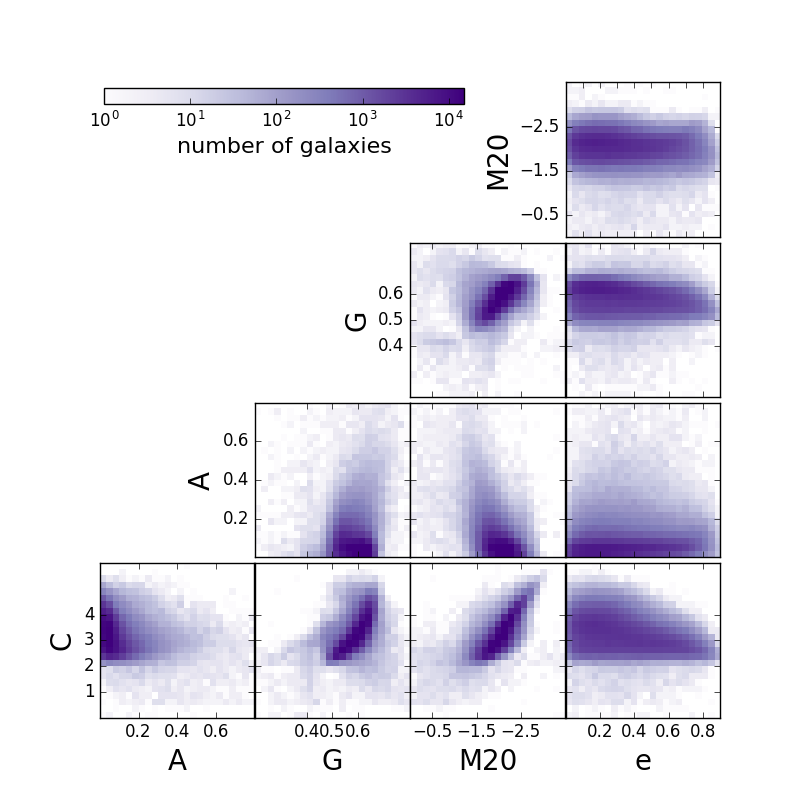
\includegraphics[width=3.65in]{figures/morph_params_entire_GZ2_sample.png}
\caption{That's a lot of parameters! \label{fig: machine classified}}
\end{figure}



%% The reference list follows the main body and any appendices.
%% Use LaTeX's thebibliography environment to mark up your reference list.
%% Note \begin{thebibliography} is followed by an empty set of
%% curly braces.  If you forget this, LaTeX will generate the error
%% "Perhaps a missing \item?".
%%
%% thebibliography produces citations in the text using \bibitem-\cite
%% cross-referencing. Each reference is preceded by a
%% \bibitem command that defines in curly braces the KEY that corresponds
%% to the KEY in the \cite commands (see the first section above).
%% Make sure that you provide a unique KEY for every \bibitem or else the
%% paper will not LaTeX. The square brackets should contain
%% the citation text that LaTeX will insert in
%% place of the \cite commands.

%% We have used macros to produce journal name abbreviations.
%% \aastex provides a number of these for the more frequently-cited journals.
%% See the Author Guide for a list of them.

%% Note that the style of the \bibitem labels (in []) is slightly
%% different from previous examples.  The natbib system solves a host
%% of citation expression problems, but it is necessary to clearly
%% delimit the year from the author name used in the citation.
%% See the natbib documentation for more details and options.


\bibliographystyle{apj}
\bibliography{apj-jour,human-machine}

%% This command is needed to show the entire author+affilation list when
%% the collaboration and author truncation commands are used.  It has to
%% go at the end of the manuscript.
%\allauthors

%% Include this line if you are using the \added, \replaced, \deleted
%% commands to see a summary list of all changes at the end of the article.
\listofchanges

\end{document}

%% End of file `sample.tex'.